\documentclass{include/protokollclass}
% Main File - Based on protokollclass.cls
% Comments are mostly in English (and some in German, concerning the Praktikum)
% ------------------------------------------------------------------------------
% Further files in folder:
%  - include/cmds.tex (for macros and additional commands)
%  - include/kitlogo.pdf (for titlepage)
%  - lit.bib (bibtex bibliography database)
%  - include/titlepage.tex (for layout of titelpage)
% ------------------------------------------------------------------------------
% Useful Supplied Packages:
% amsmath, amssymb, mathtools, bbm, upgreek, nicefrac,
% siunitx, varioref, booktabs, graphicx, tikz, multicol





%% ---------------------------------------------
%% |    Informationen über dieses Protokoll    |
%% ---------------------------------------------
\newcommand{\praktikum}{P4}                % P1 oder P2
\newcommand{\semester}{SS21}            % z.B. "WS14/15" oder "SS15"

\newcommand{\wochentag}{Mo}                % Mo, Di, Mi oder Do
\newcommand{\gruppennr}{6}                % Zweistellige Gruppennummer

\newcommand{\nachnamea}{Ahmeti}             % Nachname des ersten Praktikanten
\newcommand{\vornamea}{Dhurim}               % Vorname des ersten Praktikanten
\newcommand{\nachnameb}{Becker}              % Nachname des zweiten Praktikanten
\newcommand{\vornameb}{Alexander}              % Vorname des zweiten Praktikanten

\newcommand{\emailadressen}{uxehi@student.kit.edu; uoiyc@student.kit.edu}
% optionale Angabe von Emailadresse(n) für den Kontakt mit dem Betreuer

\newcommand{\versuch}{Laser Spectroscopy of Rubidium} % Name des Versuchs
\newcommand{\versuchsnr}{80}               % bitte die korrekte Nummer dem 
                                           % Arbeitsplatz am Versuchstag 
                                           % entnehmen
\newcommand{\fehlerrechnung}{Ja}         % Ob Fehlerrechnung im Versuch 
                                           % durchgeführt wurde oder nicht

\newcommand{\betreuer}{M. Mustermann}      % Name des zuständigen Betreuers
\newcommand{\durchgefuehrt}{19.04.2021}      % Datum, an dem der Versuch 
                                           % durchgeführt wurde





%% --------------------------------------
%% |    Settings for Word Separation    |
%% --------------------------------------
% Help for separation:
% In German package the following hints are additionally available:
% "- = Additional separation
% "| = Suppress ligation and possible separation (e.g. Schaf"|fell)
% "~ = Hyphenation without separation (e.g. bergauf und "~ab)
% "= = Hyphenation with separation before and after
% "" = Separation without a hyphenation (e.g. und/""oder)

% Describe separation hints here:
\hyphenation
{
    über-nom-me-nen an-ge-ge-be-nen
    %Pro-to-koll-in-stan-zen
    %Ma-na-ge-ment  Netz-werk-ele-men-ten
    %Netz-werk Netz-werk-re-ser-vie-rung
    %Netz-werk-adap-ter Fein-ju-stier-ung
    %Da-ten-strom-spe-zi-fi-ka-tion Pa-ket-rumpf
    %Kon-troll-in-stanz
}





% um die Titelseite per PDF-reader auszufüllen. Vorgefertigte Daten
% können in Datei 'data.tex' modifiziert werden.
%\setboolean{forminput}{true}
% um die Anmerkungen zu den Textfeldern anzeigen zu lassen
%\setboolean{showannotations}{true}
% Erneuern der Seitenzahl in jedem Kapitel
%\setboolean{chapResetPageNumb}{true}
% Einbinden der Kapitelnummer in der Seitenzahl
%\setboolean{chapWiseNumb}{true}
% english or ngerman (new german für neue deutsche Rechtschreibung statt german)
\SelectLanguage{english}





%% -----------------------
%% |    Main Document    |
%% -----------------------
\begin{document}
    % Titlepage und ToC
    \FrontMatter

    % coordinates for background border
\newcommand{\diameter}{20}
\newcommand{\xone}{-15}
\newcommand{\xtwo}{160}
\newcommand{\yone}{15}
\newcommand{\ytwo}{-253}

\newcommand{\hoehea}{60}
\newcommand{\hoeheb}{60}




\begin{titlepage}
    % background border
    \begin{tikzpicture}[overlay]
    \draw[color=gray]  
            (\xone mm, \yone mm)
      -- (\xtwo mm, \yone mm)
    arc (90:0:\diameter pt) 
      -- (\xtwo mm + \diameter pt , \ytwo mm) 
        -- (\xone mm + \diameter pt , \ytwo mm)
    arc (270:180:\diameter pt)
        -- (\xone mm, \yone mm);
    \end{tikzpicture}
    
    % KIT logo
    \begin{textblock}{10}[0,0](4.5,2.5)
        
\includegraphics[width=.25\textwidth]{include/kitlogo.pdf}
    \end{textblock}
    \changefont{phv}{m}{n}    % helvetica
    \begin{textblock}{10}[0,0](5.5,2.2)
        \begin{flushright}
            \Large FAKULTÄT FÜR PHYSIK\\Praktikum Klassische Physik
        \end{flushright}
    \end{textblock}
    
    \begin{textblock}{10}[0,0](4.2,3.1)
        \begin{tikzpicture}[overlay]
        \draw[color=gray]
            (\xone mm + 5 mm, -12 mm)
         -- (\xtwo mm + \diameter pt - 5 mm, -12 mm);
        \end{tikzpicture}
    \end{textblock}
    
    \Large
    % Zeile 1
    \begin{textblock}{12}[0,0](3.58,4.4)
        \mytextfield{Prak.}{\praktikum}{0.9cm}{17pt}
                    {P1/P2}{2}{Praktikum}
    \end{textblock}
    \begin{textblock}{12}[0,0](5.53,4.4)
        \mytextfield{Semester}{\semester}{2.6cm}{17pt}
        {z.B. \glqq WS14/15\grqq\ oder \glqq SS15\grqq}{0}{Semester}
    \end{textblock}
    \begin{textblock}{12}[0,0](9.53,4.4)
        \mytextfield{Wochentag}{\wochentag}{1.3cm}{17pt}
                    {Mo/Di/Mi/Do}{2}{Wochentag}
    \end{textblock}
    \begin{textblock}{12}[0,0](12.88,4.4)
       \mytextfield{Gruppennr.}{\gruppennr}{1.06cm}{17pt}
                   {\#\#}{2}{Gruppennummer}
    \end{textblock}
    
    % Zeile 2
    \begin{textblock}{12}[0,0](3.58,4.95)
        \mytextfield{Name}{\nachnamea}{6cm}{17pt}
                    {}{0}{Name1}
    \end{textblock}
    \begin{textblock}{12}[0,0](9.53,4.95)
        \mytextfield{Vorname}{\vornamea}{6cm}{17pt}
                    {}{0}{Vorname1}
    \end{textblock}
    
    % Zeile 3
    \begin{textblock}{12}[0,0](3.58,5.5)
        \mytextfield{Name}{\nachnameb}{6cm}{17pt}
                    {}{0}{Name2}
    \end{textblock}
    \begin{textblock}{12}[0,0](9.53,5.5)
        \mytextfield{Vorname}{\vornameb}{6cm}{17pt}
                    {}{0}{Vorname2}
    \end{textblock}
    
    % Zeile 4
    \begin{textblock}{12}[0,0](3.64,6.05)
       \normalsize\mytextfield{Emailadresse(n)}{\emailadressen}{13.1cm}{10pt}
                              {Optional}{0}{Emailadressen}
    \end{textblock}
    
    % Zeile 5
    \begin{textblock}{12}[0,0](3.58,7)
        \mytextfield{Versuch}{\versuch\ (\praktikum-\versuchsnr)}{9.45cm}{14pt}
                    {z.B. \glqq Galvanometer (P1-13)\grqq\ oder \glqq %
                     Mikrowellenoptik (P2-15)\grqq}{0}{Versuch}
    \end{textblock}
    \begin{textblock}{12}[0,0](12.58,7)
       \mytextfield{Fehlerrech.}{\fehlerrechnung}{1.46cm}{17pt}
                   {Ja/Nein}{4}{Fehlerrechnung}
    \end{textblock}
    
    % Zeile 6
    \begin{textblock}{12}[0,0](3.58,7.55)
        \mytextfield{Betreuer}{\betreuer}{7cm}{17pt}{}{0}{Betreuer}
    \end{textblock}
    \begin{textblock}{12}[0,0](10.82,7.55)
        \mytextfield{Durchgeführt am}{\durchgefuehrt}{2.53cm}{17pt}
                    {TT.MM.JJ}{8}{Durchfuehrung}
    \end{textblock}
    
    % Querstrich
    \begin{textblock}{20}[0,0](0,7.9)\tiny\centering
        Wird vom Betreuer ausgefüllt.
    \end{textblock}
    \begin{tikzpicture}[overlay]
    \draw[color=gray]
        (\xone mm + 5 mm, -95 mm)
     -- (\xtwo mm + \diameter pt - 5 mm, -95 mm);
    \end{tikzpicture}
    
    % Zeile 1
    \begin{textblock}{12}[0,0](3.65,8.57)
        \myTtextfield{1. Abgabe am}{}{2.5cm}{17pt}
                     {}
    \end{textblock}
    
    % Block 1
    \begin{tikzpicture}[overlay]
    \draw[color=gray]  
        (\xone mm + 10 mm, -107.5 mm)
     -- (\xtwo mm + \diameter pt - 10 mm, -107.5 mm)
     -- (\xtwo mm + \diameter pt - 10 mm, -107.5 mm - \hoehea mm)
     -- (\xone mm + 10 mm, -107.5 mm - \hoehea mm)
     -- (\xone mm + 10 mm, -107.5 mm);
    \end{tikzpicture}
    \begin{textblock}{20}[0,0](3.8,9.2)
        \myTtextfield{Rückgabe am}{}{2.5cm}{17pt}
                     {}
    \end{textblock}
    \begin{textblock}{20}[0,0](8.7,9.2)
        \smash{Begründung:}
    \end{textblock}
    
    % Zeile 2
    \begin{textblock}{12}[0,0](3.65,12.6)
        \myTtextfield{2. Abgabe am}{}{2.5cm}{17pt}
                     {}
    \end{textblock}
    
    % Block 2
    \begin{tikzpicture}[overlay]
    \draw[color=gray]  
        (\xone mm + 10 mm, -180 mm)
     -- (\xtwo mm + \diameter pt - 10 mm, -180 mm)
     -- (\xtwo mm + \diameter pt - 10 mm, -180 mm - \hoehea mm)
     -- (\xone mm + 10 mm, -180 mm - \hoehea mm)
     -- (\xone mm + 10 mm, -180 mm);
    \end{tikzpicture}
    \begin{textblock}{12}[0,0](4,13.25)
        \smash{Ergebnis:~~~~+~~~/~~~0~~~/~~~-}
    \end{textblock}
    \begin{textblock}{12}[0,0](9.5,13.25)
        \smash{Fehlerrechnung:~~~Ja~~~/~~~Nein}
    \end{textblock}
    \begin{textblock}{12}[0,0](3.8,13.72)
        \myTtextfield{Datum}{}{2.5cm}{17pt}
                     {}
    \end{textblock}
    \begin{textblock}{12}[0,0](8.3,13.72)
        \myTtextfield{Handzeichen}{}{5.5cm}{17pt}
                     {}
    \end{textblock}
    \begin{textblock}{12}[0,0](4,14.25)\Large
        \smash{Bemerkungen:}
    \end{textblock}
    
    
    
    % lowest text blocks concerning the KIT
    \begin{textblock}{10}[0,0](4,16.8)
        \tiny{KIT -- Universität des Landes Baden-Württemberg und nationales %
              Forschungszentrum in der Helmholtz-Gemeinschaft}
    \end{textblock}
    \begin{textblock}{10}[0,0](14,16.75)
        \large{\textbf{www.kit.edu}}
    \end{textblock}
\end{titlepage}
 %\cleardoublepage

    \begingroup \let\clearpage\relax    % in order to avoid listoffigures and
    \tableofcontents                    % listoftables on new pages
    \listoffigures
    \listoftables
    \endgroup
    %\cleardoublepage



    % Contents
    \MainMatter
    \chapter{Written preparation}

\textbf{Q}: How strong can the excited state of a two-level system be populated and what happens in the limit of infinitely strong laser intensities? \\
\textbf{A}: A two level system can be populated up to parity between the levels. Increasing laser input power only increases the rate of relaxation.\\
\\
\noindent
\textbf{Q}: What are the physical causes of the fine and hyperfine splitting? \\
\textbf{A}: Fine splitting: i) Relativistic mass increase ii) Darwin term iii) Mutual coupling of magnetic moment of electron spin $\vec{\mu}_{s}$ and magnetic field associated with orbital movement of electron $\vec{B}_{l}$. Hyperfine splitting: i) Finite size of nucleus ii) Coupling of $\vec{\mu}_{I}$ and $\vec{B}_{j}$.\\
\\
\noindent
\textbf{Q}: How much smaller is the hyperfine splitting compared to the fine splitting? \\
\textbf{A}: $\frac{\Delta E_{hf}}{\Delta E_{f}}=\frac{\vec{\mu}_{I}}{\vec{\mu}_{s}}=\frac{m_{e}}{m_{n}}=\frac{1}{1836}$.\\
\\
\noindent
\textbf{Q}: Why is only the $D_{2}$ line in the focus of this experiment? \\
\textbf{A}: Because the $D_{1}$ line with $\lambda=794.98nm$ is not accessible with the laser used with a wavelength range of $778.99nm-788.4nm$.\\
\\
\noindent
\textbf{Q}: Which parameters influence the free spectral range and the spectral linewidth of a resonator? \\
\textbf{A}: $FSR\sim\frac{c_{0}}{nl}$ and $\Delta\nu\sim\frac{c_{0}}{nl}\mathcal{F}^{-1}$.\\
\\
\noindent
\textbf{Q}: Why is it impossible to build a laser with a laser medium based on two-level sys- tems? \\
\textbf{A}: Because a state inversion is not possibile in a two level system.\\
\\
\noindent
\textbf{Q}: How can the laser wavelength be tuned? \\
\textbf{A}: i) Rotation of diffraction grating ii) Change of temperatur $T$ of laser medium iii) Change of injection current $I_{in}$ of laser diode.\\
\\
\noindent
\textbf{Q}: Which tuning method can be attributed to coarse tuning, which to fine tuning? \\
\textbf{A}: Rotation of the diffraction grating can be attributed to coarse tuning and the rest to fine tuning.\\
\\
\noindent
\textbf{Q}: How fast are the tuning methods compared to each other? \\
\textbf{A}: Tuning by the rotation of the diffraction grating is faster.\\
\\\\
\noindent
\textbf{Q}: How is the intensity of a semiconductor laser usually changed? \\
\textbf{A}: Through placing of neutral density filters into the beam path and rotating of the $\lambda/2$-retarder.\\
\\
\noindent
\textbf{Q}: How does the signal after the reference resonator look like if the laser wavelength is continuously tuned? \\
\textbf{A}: It looks like in figure \ref{fig:Intres.}.\\
\\
\noindent
\textbf{Q}: Which transitions contribute to the D2 line of Rubidium? \\
\textbf{A}: $^{85}Rb$, $5^{2}s_{1/2}\leftrightarrow5^{2}p_{3/2}$: $F=2\leftrightarrow F=1$, $F=2\leftrightarrow F=2$, $F=2\leftrightarrow F=3$, $F=3\leftrightarrow F=2$, $F=3\leftrightarrow F=3$, $F=3\leftrightarrow F=4$.\\
$^{87}Rb$, $5^{2}s_{1/2}\leftrightarrow5^{2}p_{3/2}$: $F=1\leftrightarrow F=0$, $F=1\leftrightarrow F=1$, $F=1\leftrightarrow F=2$, $F=2\leftrightarrow F=1$, $F=2\leftrightarrow F=2$, $F=2\leftrightarrow F=3$.\\
\\
\noindent
\textbf{Q}: Which spectral lines can still be resolved with the common absorption spectroscopy technique and why? \\
\textbf{A}: Some of the hyperfine spectral lines can still be resolved because their difference is bigger than $1 GHz$, which is the order of the Doppler broadening at room temperature.\\
\\
\noindent
\textbf{Q}: Which lines are usually stronger, the main saturated absorption peaks or the crossover peaks? \\
\textbf{A}: The main saturated absorption peaks are usually stronger.

\chapter{Aim of the experiment, theoretical basics}
Optical spectroscopy is a useful method for many reasons. With its assistance it is possible for example to study the interaction between electromagnetic radiation and matter, to detect atoms and molecules and to identify them. In the experiment under consideration we carry out an quantitive investigation of the hyper fine structure of rubidium. The exact techniques we take advantage of for that, are the \textbf{absorption spectroscopy} and the \textbf{Doppler-free saturation spectroscopy}.

Before we dive into the details of the experiment itself, we need to take a look at the theory behind it. For the interaction between an atom or molecule and light to be possible, the resonance condition

\begin{equation}
\label{E:Res. con.}
E_2-E_1=h\nu
\end{equation}

\noindent
needs to be fulfilled. 

If such an event takes place, we can distinguish between three different cases: \textbf{absorption}, \textbf{stimulated emission} and \textbf{spontaneous emission}. Through absorption an electron is excited from a lower energy level $E_1$ to an higher one $E_2$. During stimulated emission on the other hand an already excited electron at the energy $E_2$ falls upon interaction with a photon of appropriate frequency to a lower lying level $E_1$. In the process an additional photon is created, which travels in the same direction as the stimulating one. When an electron in an excited state of an atom or molecule falls to a lower state without the presence of any light, we talk about spontaneous emission. All three processes are shown schematically in figure \ref{fig:Emisabs.}.

\begin{figure}[h]
    \centering
    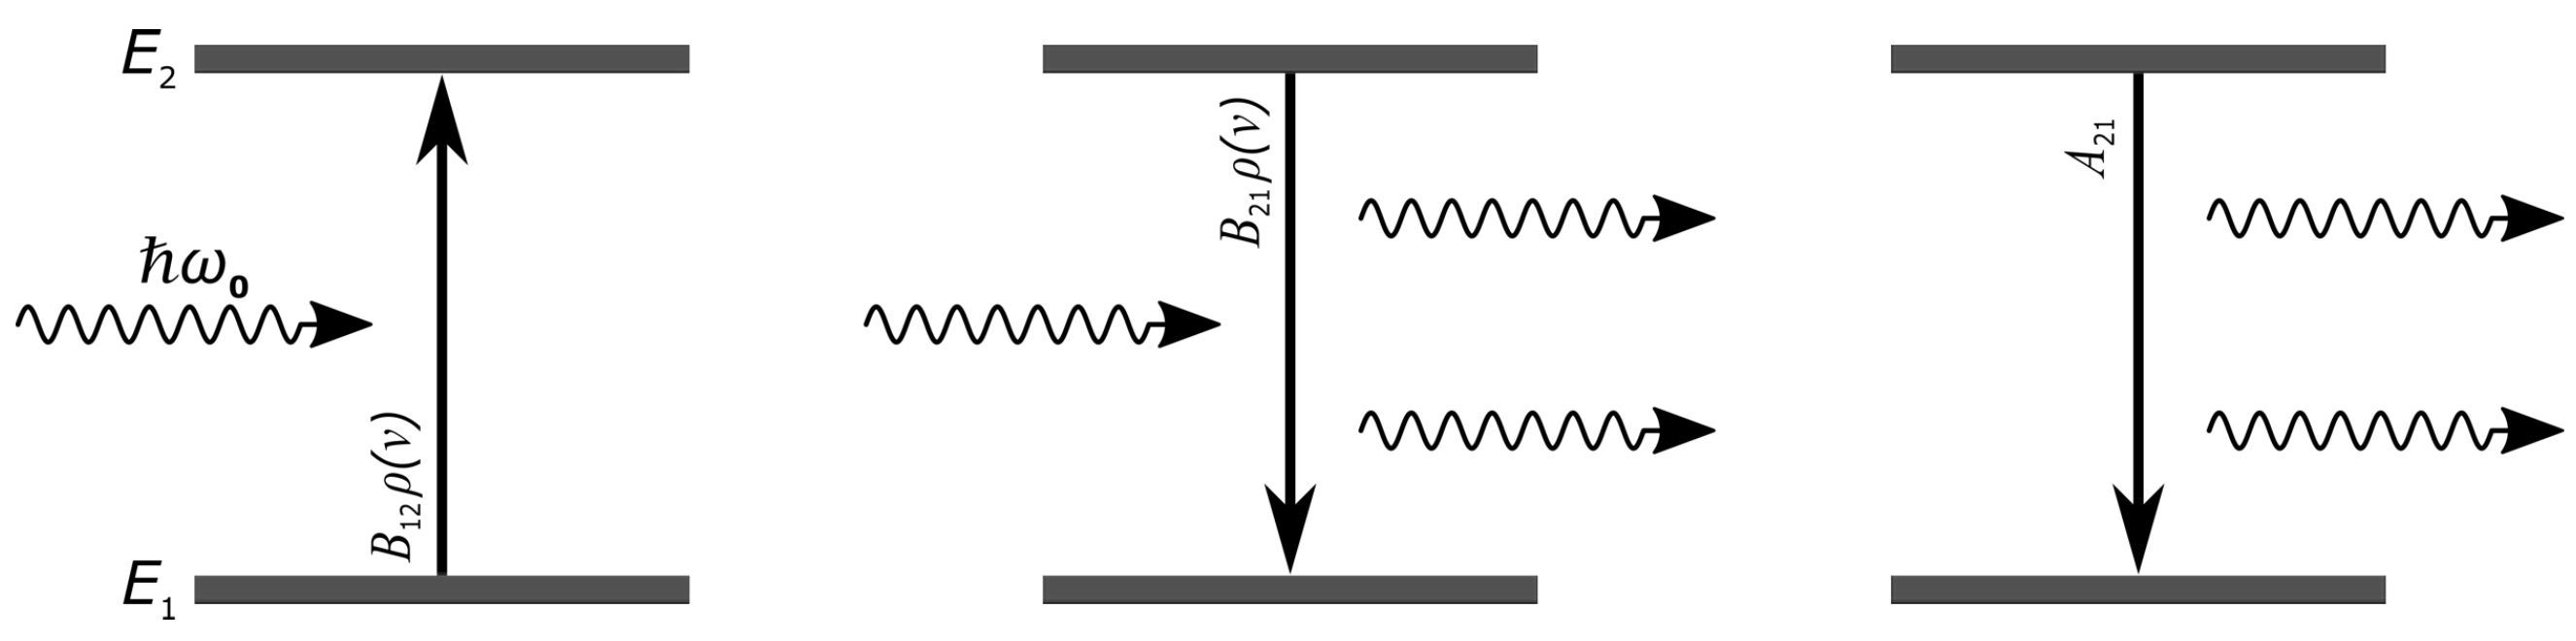
\includegraphics[width=15.8cm]{Emisabs.png}
    \caption{Illustration of absorption, stimulated emission and spontaneous emission.}
    \label{fig:Emisabs.}
\end{figure}

When we look out for the hyper fine lines in the spectrum of rubidium, we have to consider that this task is made more difficult by the fact that the absorption lines have a finite linewidth. The phenomena associated with this are the \textbf{natural linewidth}, \textbf{collisional broadening}, \textbf{Doppler broadening} and \textbf{saturation broadening}. The cause of the natural linewidth is Heisenberg's uncertainty principle including the quantities energy $E$ and time $t$. As we can conclude from the already mentioned event of spontaneous emission, an excited state has a finite lifetime $\tau$. This is correlated with a certain energitical uncertainty $\Delta E$ of the corresponding transition. The energy is again related to the frequency through $\Delta E=\hbar \Delta \omega$, which is exactly the natural lindewidth we can see in a recorded spectrum. The line profile we get from this kind of broadening has a Lorentzian shape. In the case of collisional broadening we have to differentiate between elastic and inelastic collisions. During elastic collisions there is no transfer of energy between the two regarded particles, but to the electromagnetic radiation field. This leads to uncorrelated emission processes, whose durations are Poisson distributed around the mean free time. In other words, we have a broadening and shift of the atoms` spectral lines. The mechanism is different for inelastic collisions: The excited electrons of the interacting atoms are given an additional way of relaxation, what causes a shortening of the according lifetime. Like it is with the natural linewidth, this has because of the uncertainty principle a broadening effect. Doppler broadening is obviously based on the Doppler effect, described by the relation

\begin{equation}
\label{E:Dopp.}
\omega'=\omega_{0}\left(1-\frac{v_{z}}{c}\right).
\end{equation}

\noindent
As we know, the velocities $v_{z}$ are distributed corresponding to the Maxwell-Boltzmann distribution. Thus the according line shape is of Gaussian character. Under usual ambient conditions the Doppler broadening is two orders of magnitudes larger than the natural broadening. But if we have a similar contribution of the former two, then the overlapping generates a Voigt profile. All of the previously stated facts are graphically shown in figure \ref{fig:Dopp.}.

\begin{figure}[h]
    \centering
    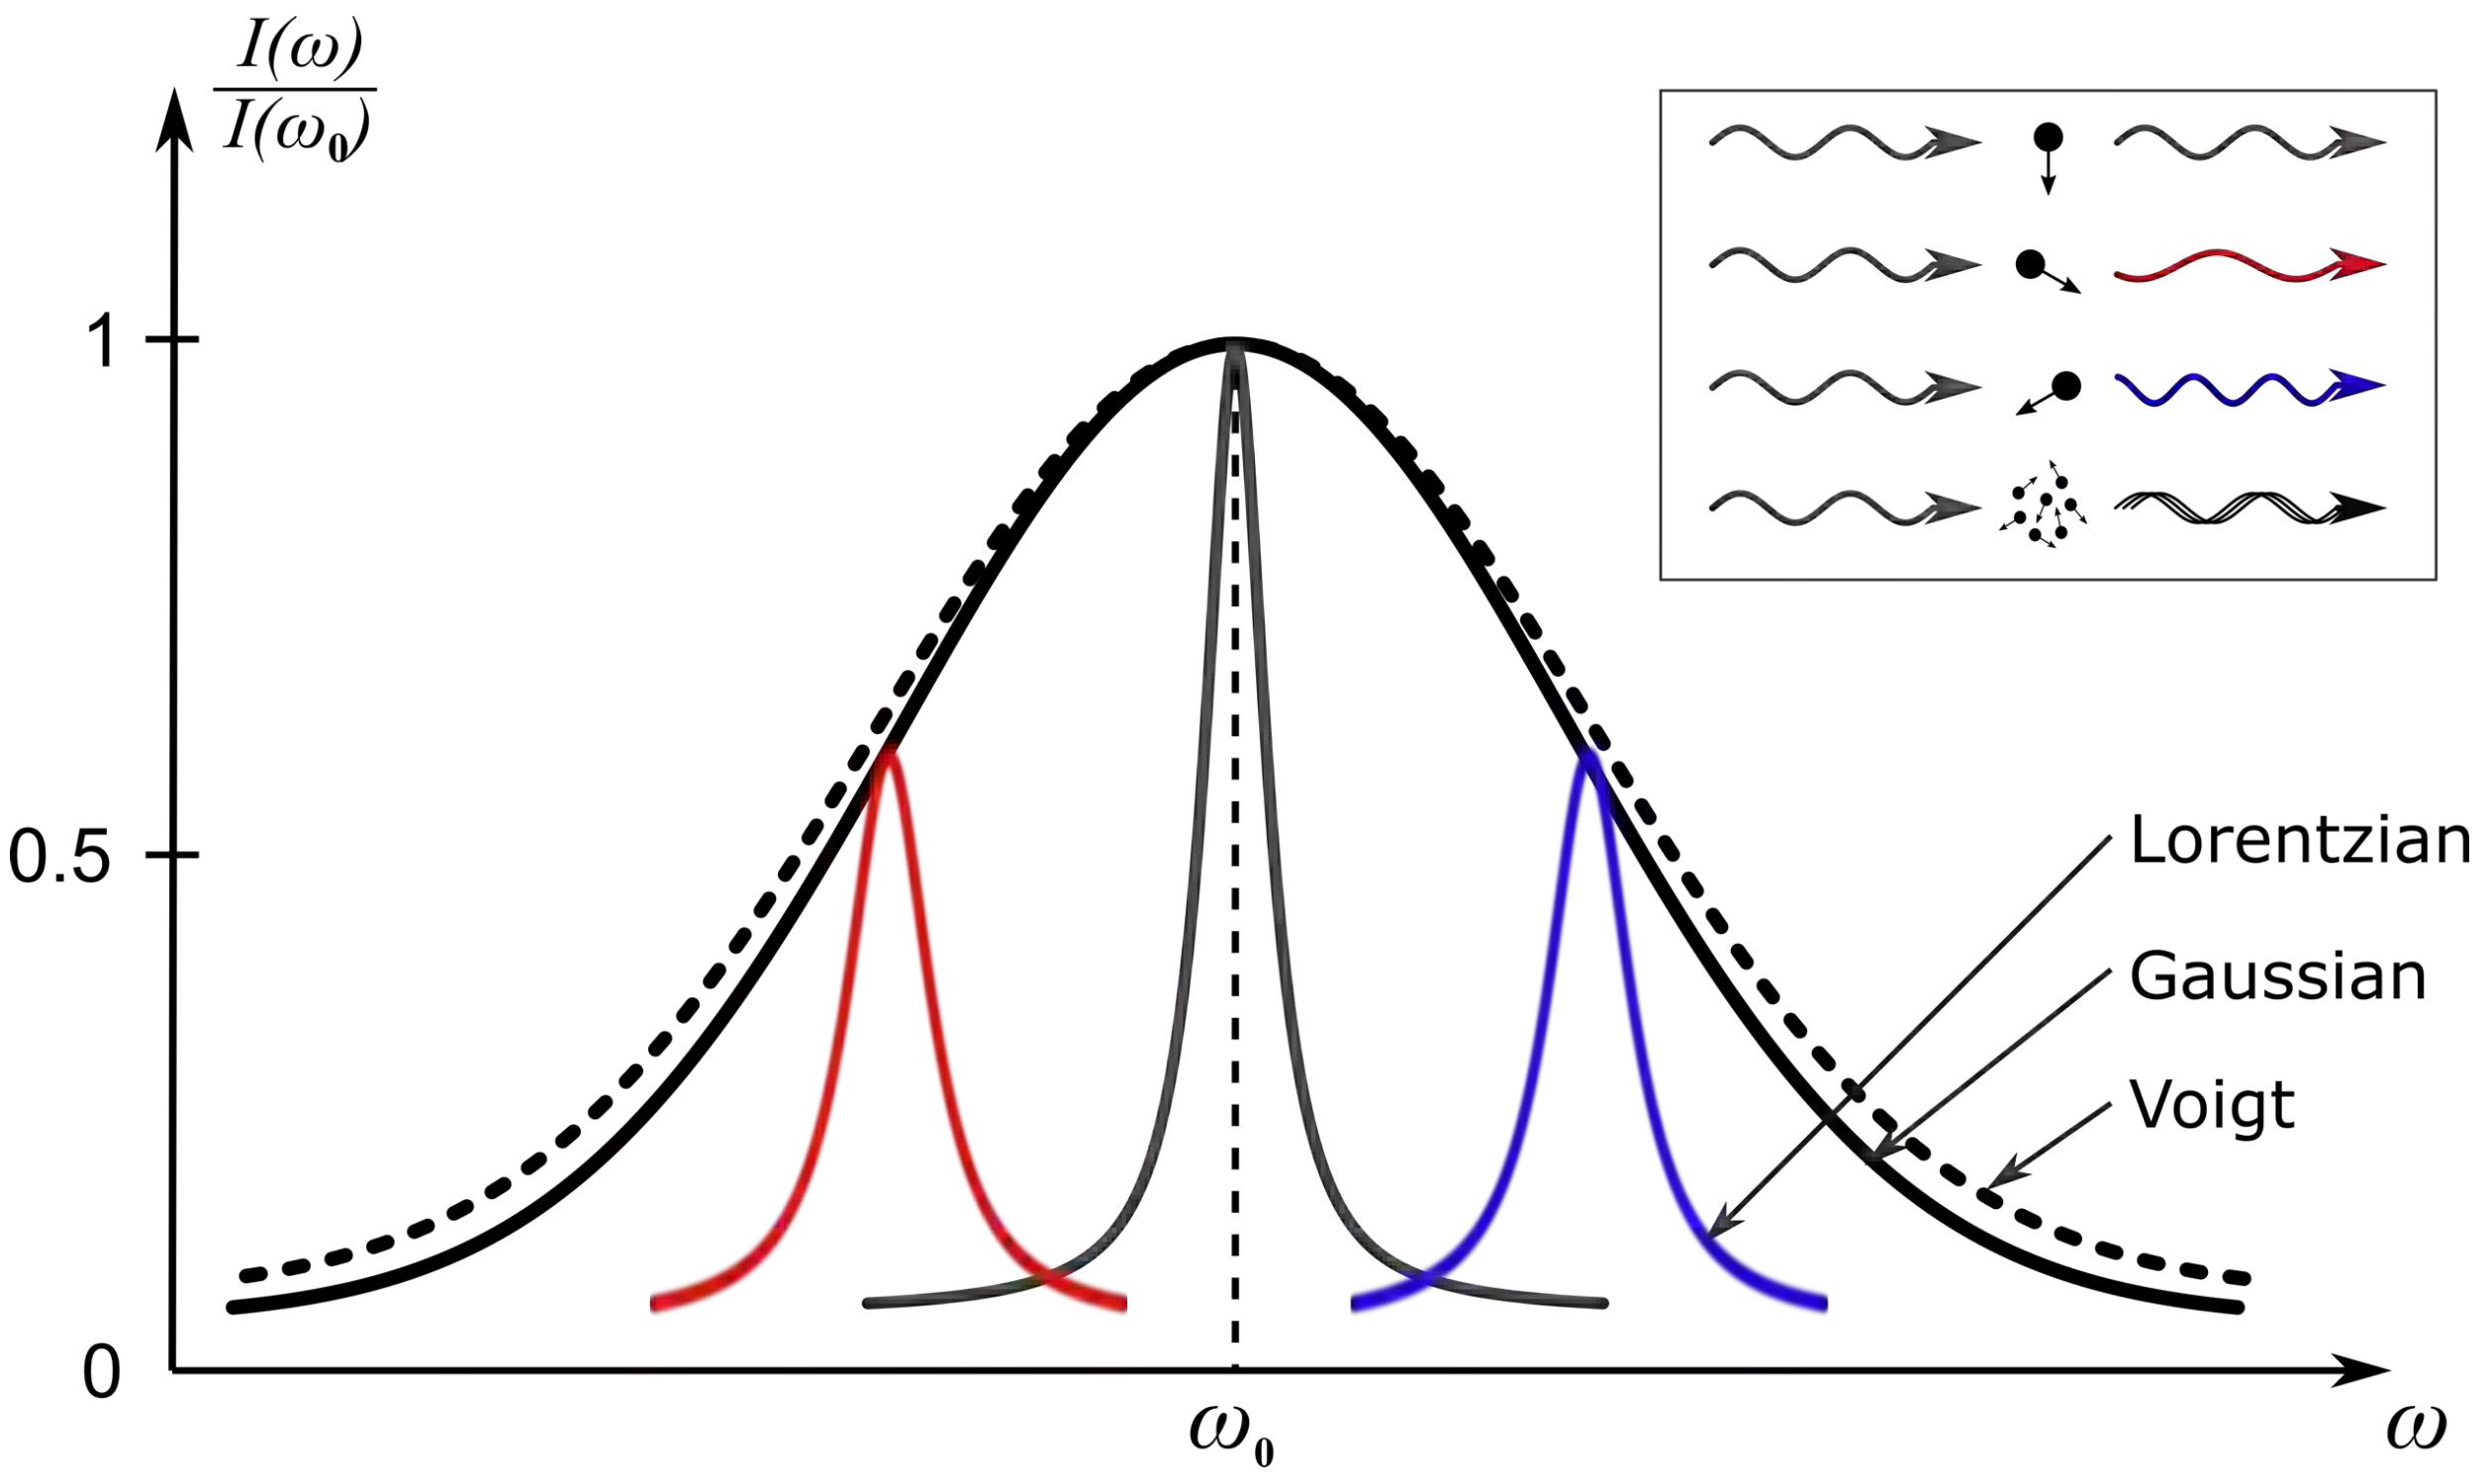
\includegraphics[width=10cm]{Dopp.png}
    \caption{Resulting line shapes due to natural broadening and Doppler broadening.}
    \label{fig:Dopp.}
\end{figure}

\noindent
What happens while saturation broadening is basically the following: We get an additional (partial) saturation of the wing-frequencies in the finite width of the atomic energy levels and the frequency interval of the laser.

As already mentioned, the spectrum, which we'll be looking at, stems from the alkali metal rubidium Rb. But what also has to be taken into account is, that rubidium has two different isotopes: About $72.17\%$ of its natural abundance is $^{85}Rb$ and $27.83\%$ $^{87}Rb$. This results in a so called \textbf{isotopic shift} between the hyper fine lines of those two. Since the properties like spin, mass, volume and charge distribution of the respective nuclei are different, we get this additional shift (see figure \ref{fig:term.}).

\begin{figure}[h]
    \centering
    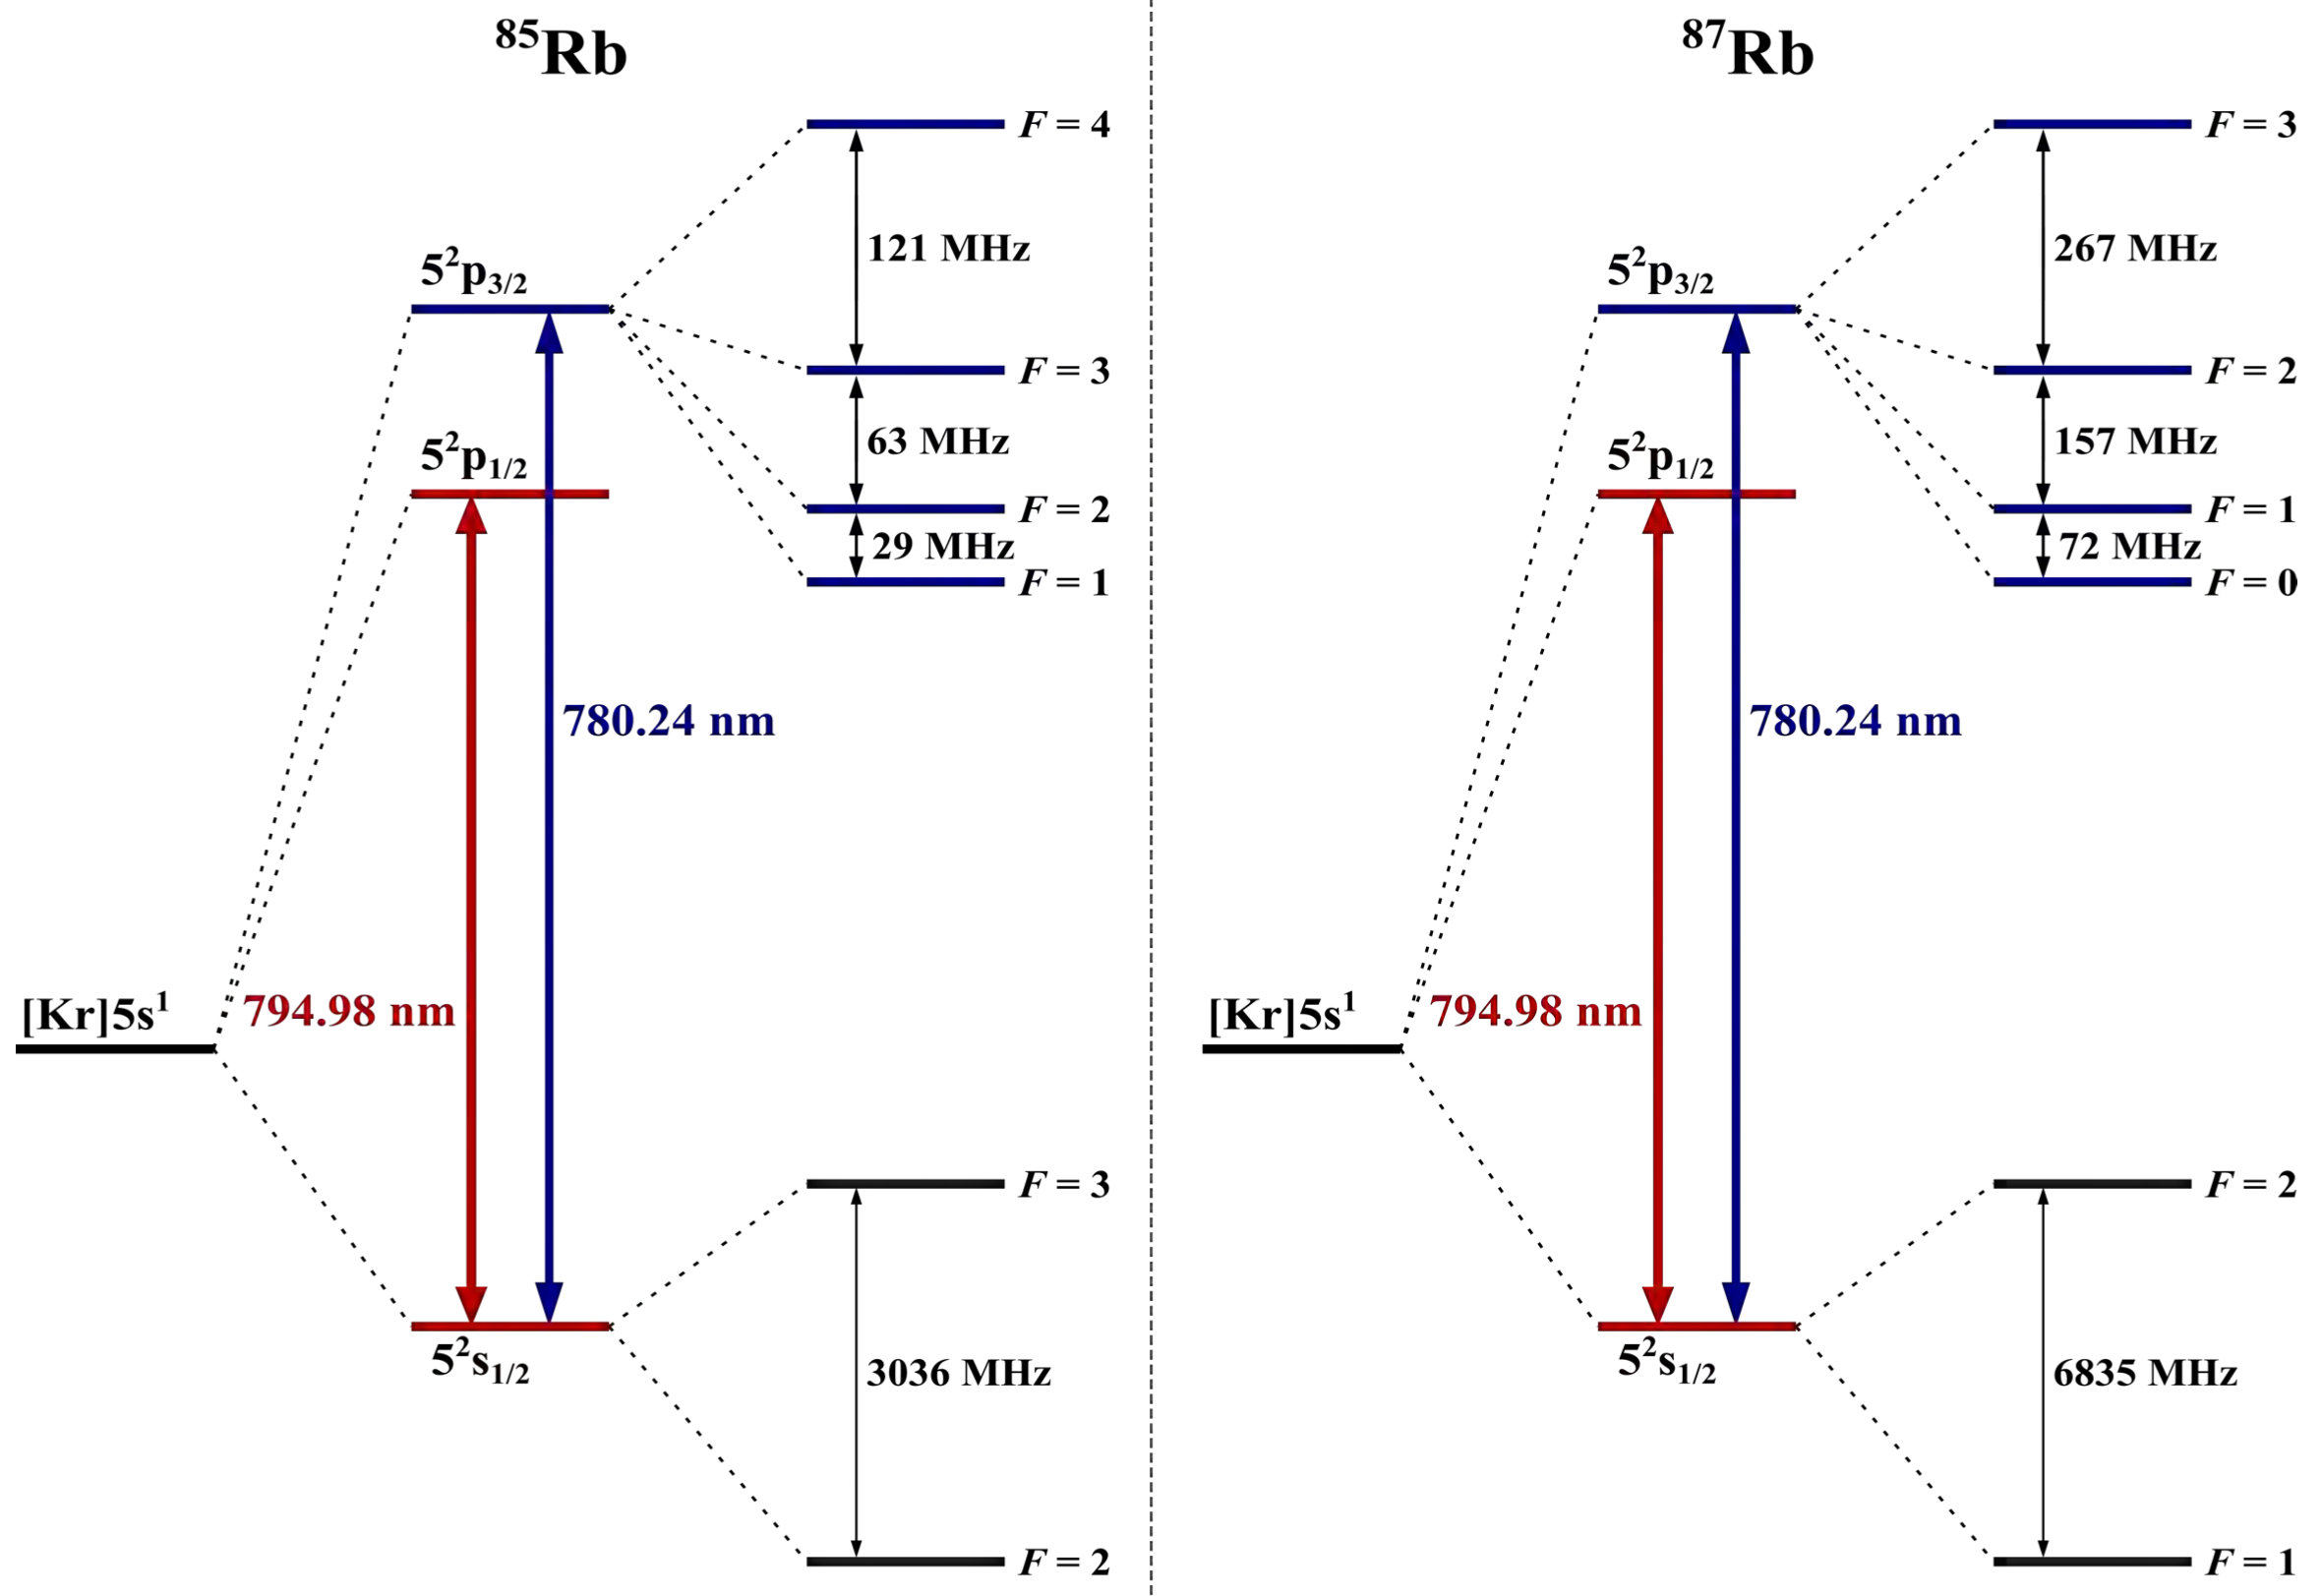
\includegraphics[width=15.8cm]{term.png}
    \caption{Term diagram of $^{85}Rb$ and $^{87}Rb$. The transition highlighted in red is the $D_{1}$ transition and the one in blue the $D_{2}$ transition.}
    \label{fig:term.}
\end{figure}

Not all transitions between hyper fine levels, that one could think of, are possibile. One has to keep in mind, that the selection rules have to be followed:

\begin{equation}
\label{E:Deltas}
\Delta s=0,
\end{equation}

\begin{equation}
\label{E:Deltal}
\Delta l=\pm1,
\end{equation}

\begin{equation}
\label{E:Deltaj}
\Delta j=0,\pm1 \;\; \text{except} \;\; j=0\leftrightarrow j=0,
\end{equation}

\begin{equation}
\label{E:DeltaF}
\Delta F=0,\pm1 \;\; \text{except} \;\; F=0\leftrightarrow F=0.
\end{equation}

\begin{figure}[h]
    \centering
    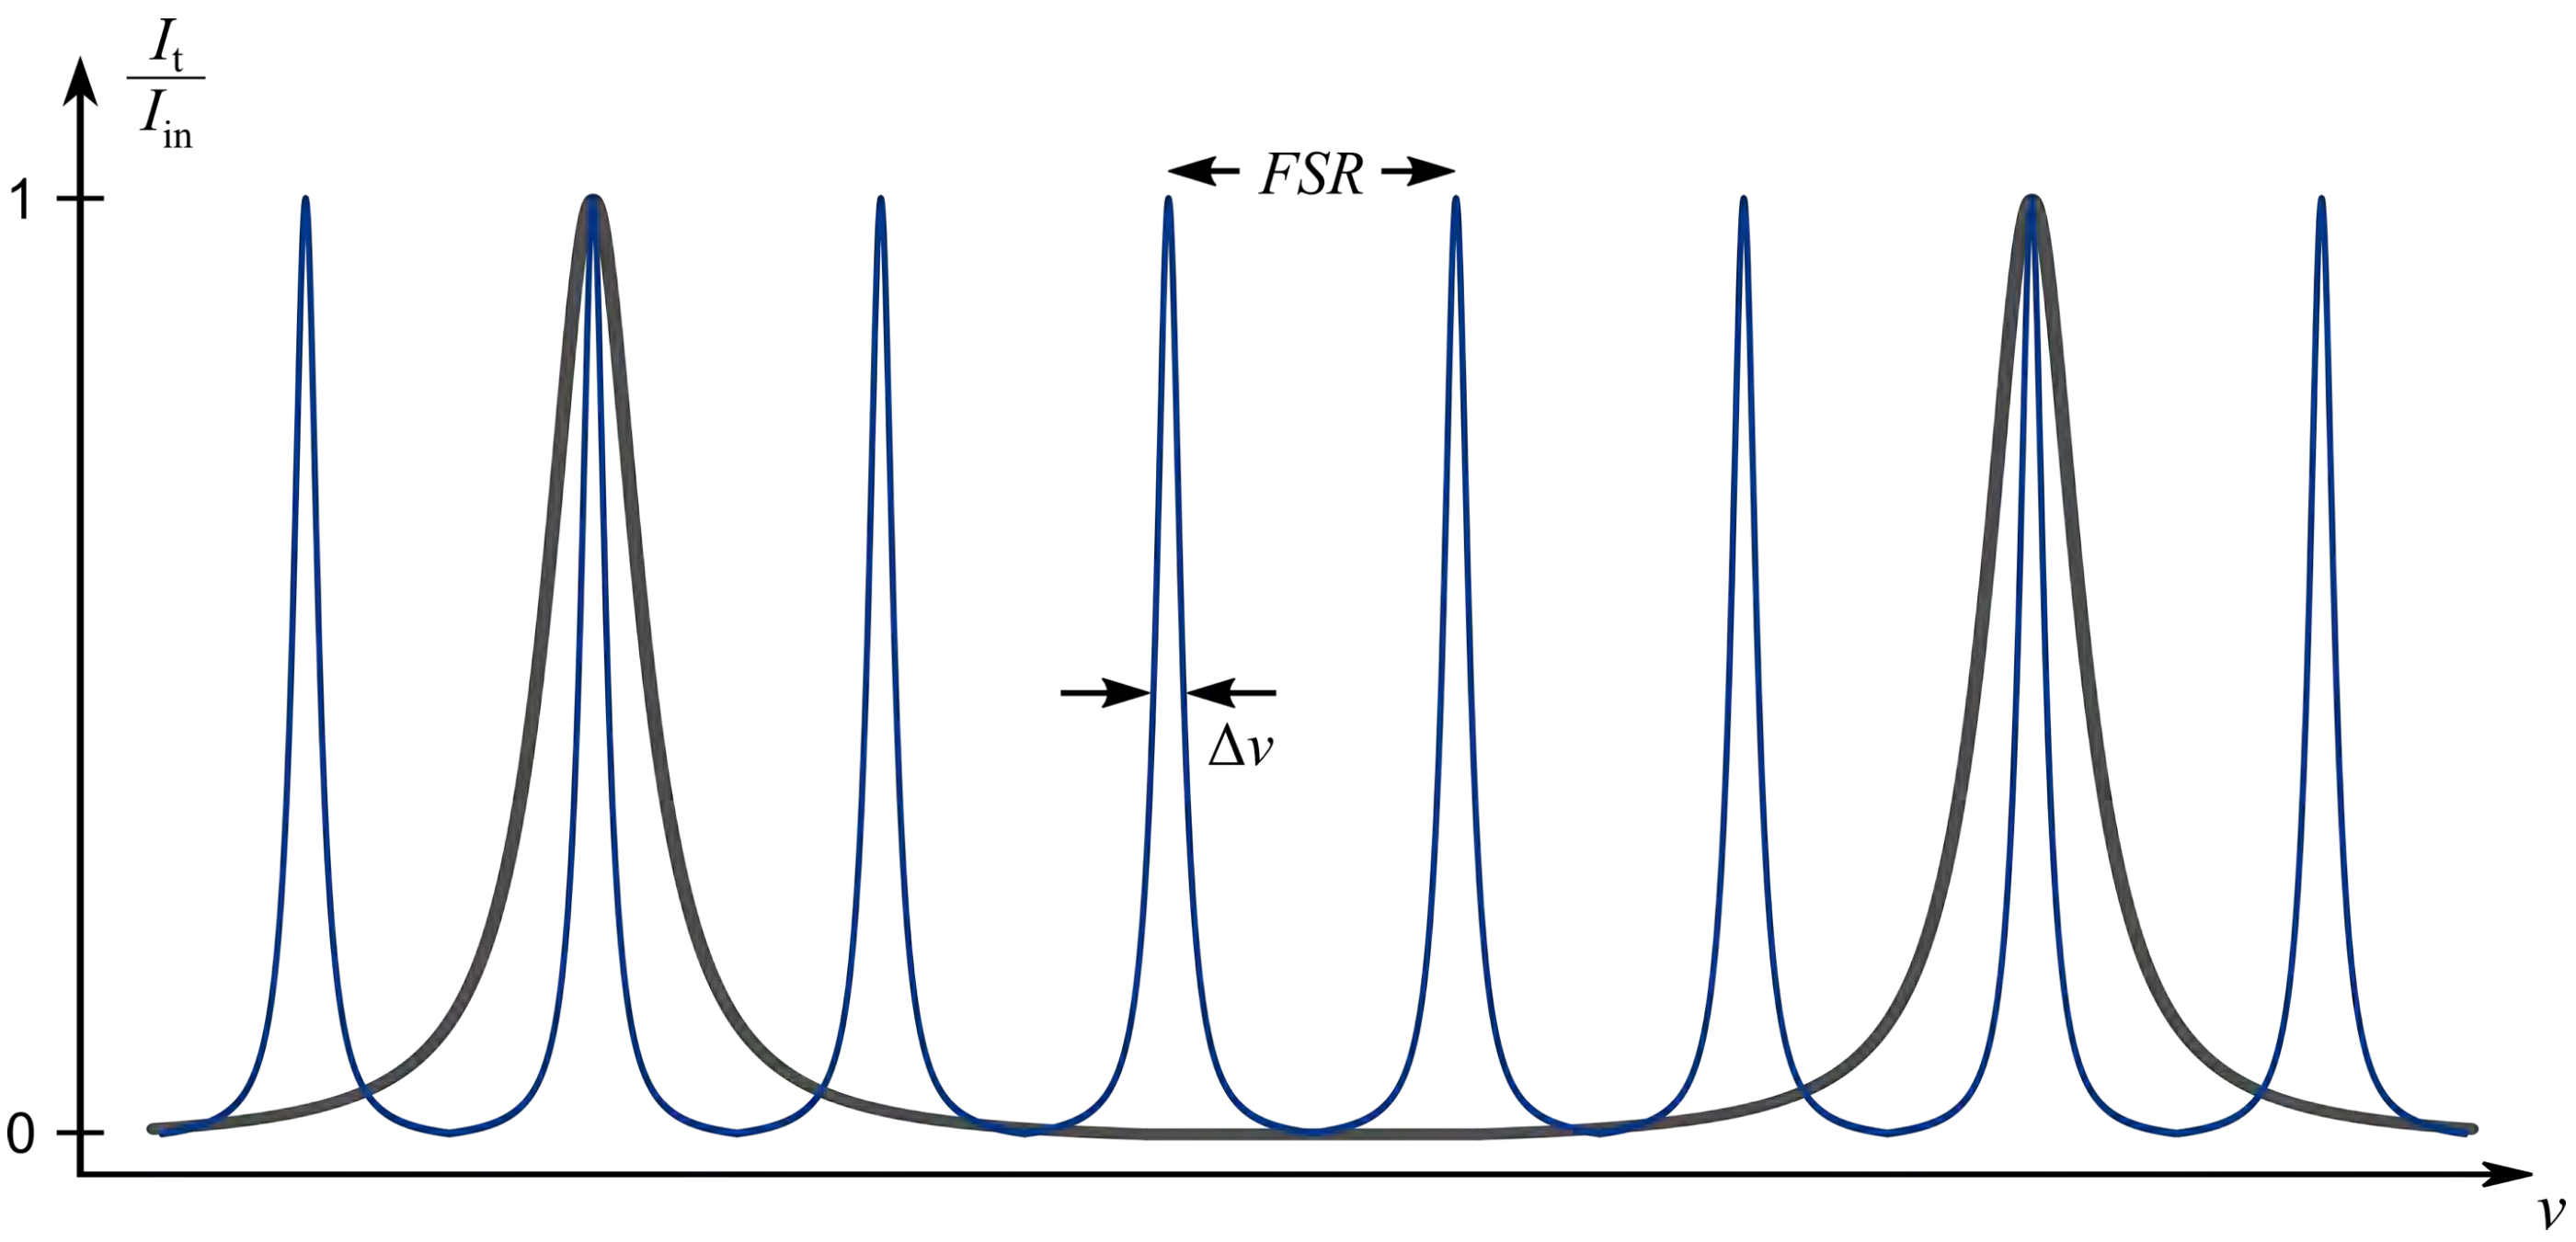
\includegraphics[width=13cm]{Intres.png}
    \caption{Transmitted intensity as a function of frequency. The gray curve stands for the eigenmodes of a resonator of $F\approx30$. The blue eigenmodes on the other hand belong to a resonator of same finesse but five times the length.}
    \label{fig:Intres.}
\end{figure}

Now that we know about the properties of our rubidium atoms and their interaction with light, which are important for the understanding of the experiment, we can learn about how some devices, used in the experiment, work in principle. First we'll discuss the \textbf{Fabry-Pérot resonator}. It consists of two opposing mirrors with distance $l$. When light enters from one side, it gets reflected multiple times and it forms a standing wave. The resonance condition for the wavelength is

\begin{equation}
\label{E:Deltaj}
\lambda_{m}=\frac{2l}{m} \;\; m \in \mathbb{N}.
\end{equation}

\noindent
The equivalent condition for the frequency is

\begin{equation}
\label{E:Deltaj}
\nu_{m}=\frac{c}{2l}m,
\end{equation}

\noindent
That means that there exists a certain distance in the frequency space between two adjacent resonator modes. This quantity is called \textbf{free spectral range}:

\begin{equation}
\label{E:Deltaj}
FSR=\nu_{m}-\nu_{m-1}=\frac{c_{0}}{2nl},
\end{equation}

\noindent
where $c_{0}$ is the speed of light in vacuum and $n$ the index of refraction. Also the $FSR$ indicates the cycle frequency of the light in the resonator. Related to that is another quantity of interest, which is called \textbf{finesse}:

\begin{equation}
\label{E:Deltaj}
\mathcal{F}=\frac{FSR}{\Delta\nu}=\frac{\pi\sqrt{R}}{1-R}.
\end{equation}

\noindent
As can be seen, it depends solely on the resonator's losses. That means for the spectral line width

\begin{equation}
\label{E:speclinwid}
\Delta\nu=\gamma=\frac{c_{0}}{2nl}\mathcal{F}^{-1}.
\end{equation}

\noindent
How the amount of the transmitted intensity in relation to the incoming intensity of the light $\frac{I_{t}}{I_{in}}$ depends on said quantities for different values of the frequency $\nu$ is demonstrated in figure \ref{fig:Intres.}. 

A problem with the ordinary Fabry-Pérot resonator is that after a slight misalignment of the direction of the light the electromagnetic wave leaves the space between the mirrors pretty quickly. The corrective is a \textbf{confocal resonator}. The used mirrors now posses a finite curvature $r=2f$ for more stability. The distance between them is set to $l=2f$. A look at figure \ref{fig:Confres.} makes it clear, that the path length of the light changes to double the amount. Consequently we get a change of the formulas of our resonance condition to

\begin{equation}
\label{E:Deltaj}
\lambda_{m}=\frac{4l}{m}	\;\; m \in \mathbb{N},
\end{equation}

\noindent
the free spectral range to

\begin{equation}
\label{E:Deltaj}
FSR=\frac{c_{0}}{4nl},
\end{equation}

\noindent
and the finesse to

\begin{equation}
\label{E:Deltaj}
\mathcal{F}=\frac{\pi R}{1-R^{2}}.
\end{equation}

\begin{figure}[h]
    \centering
    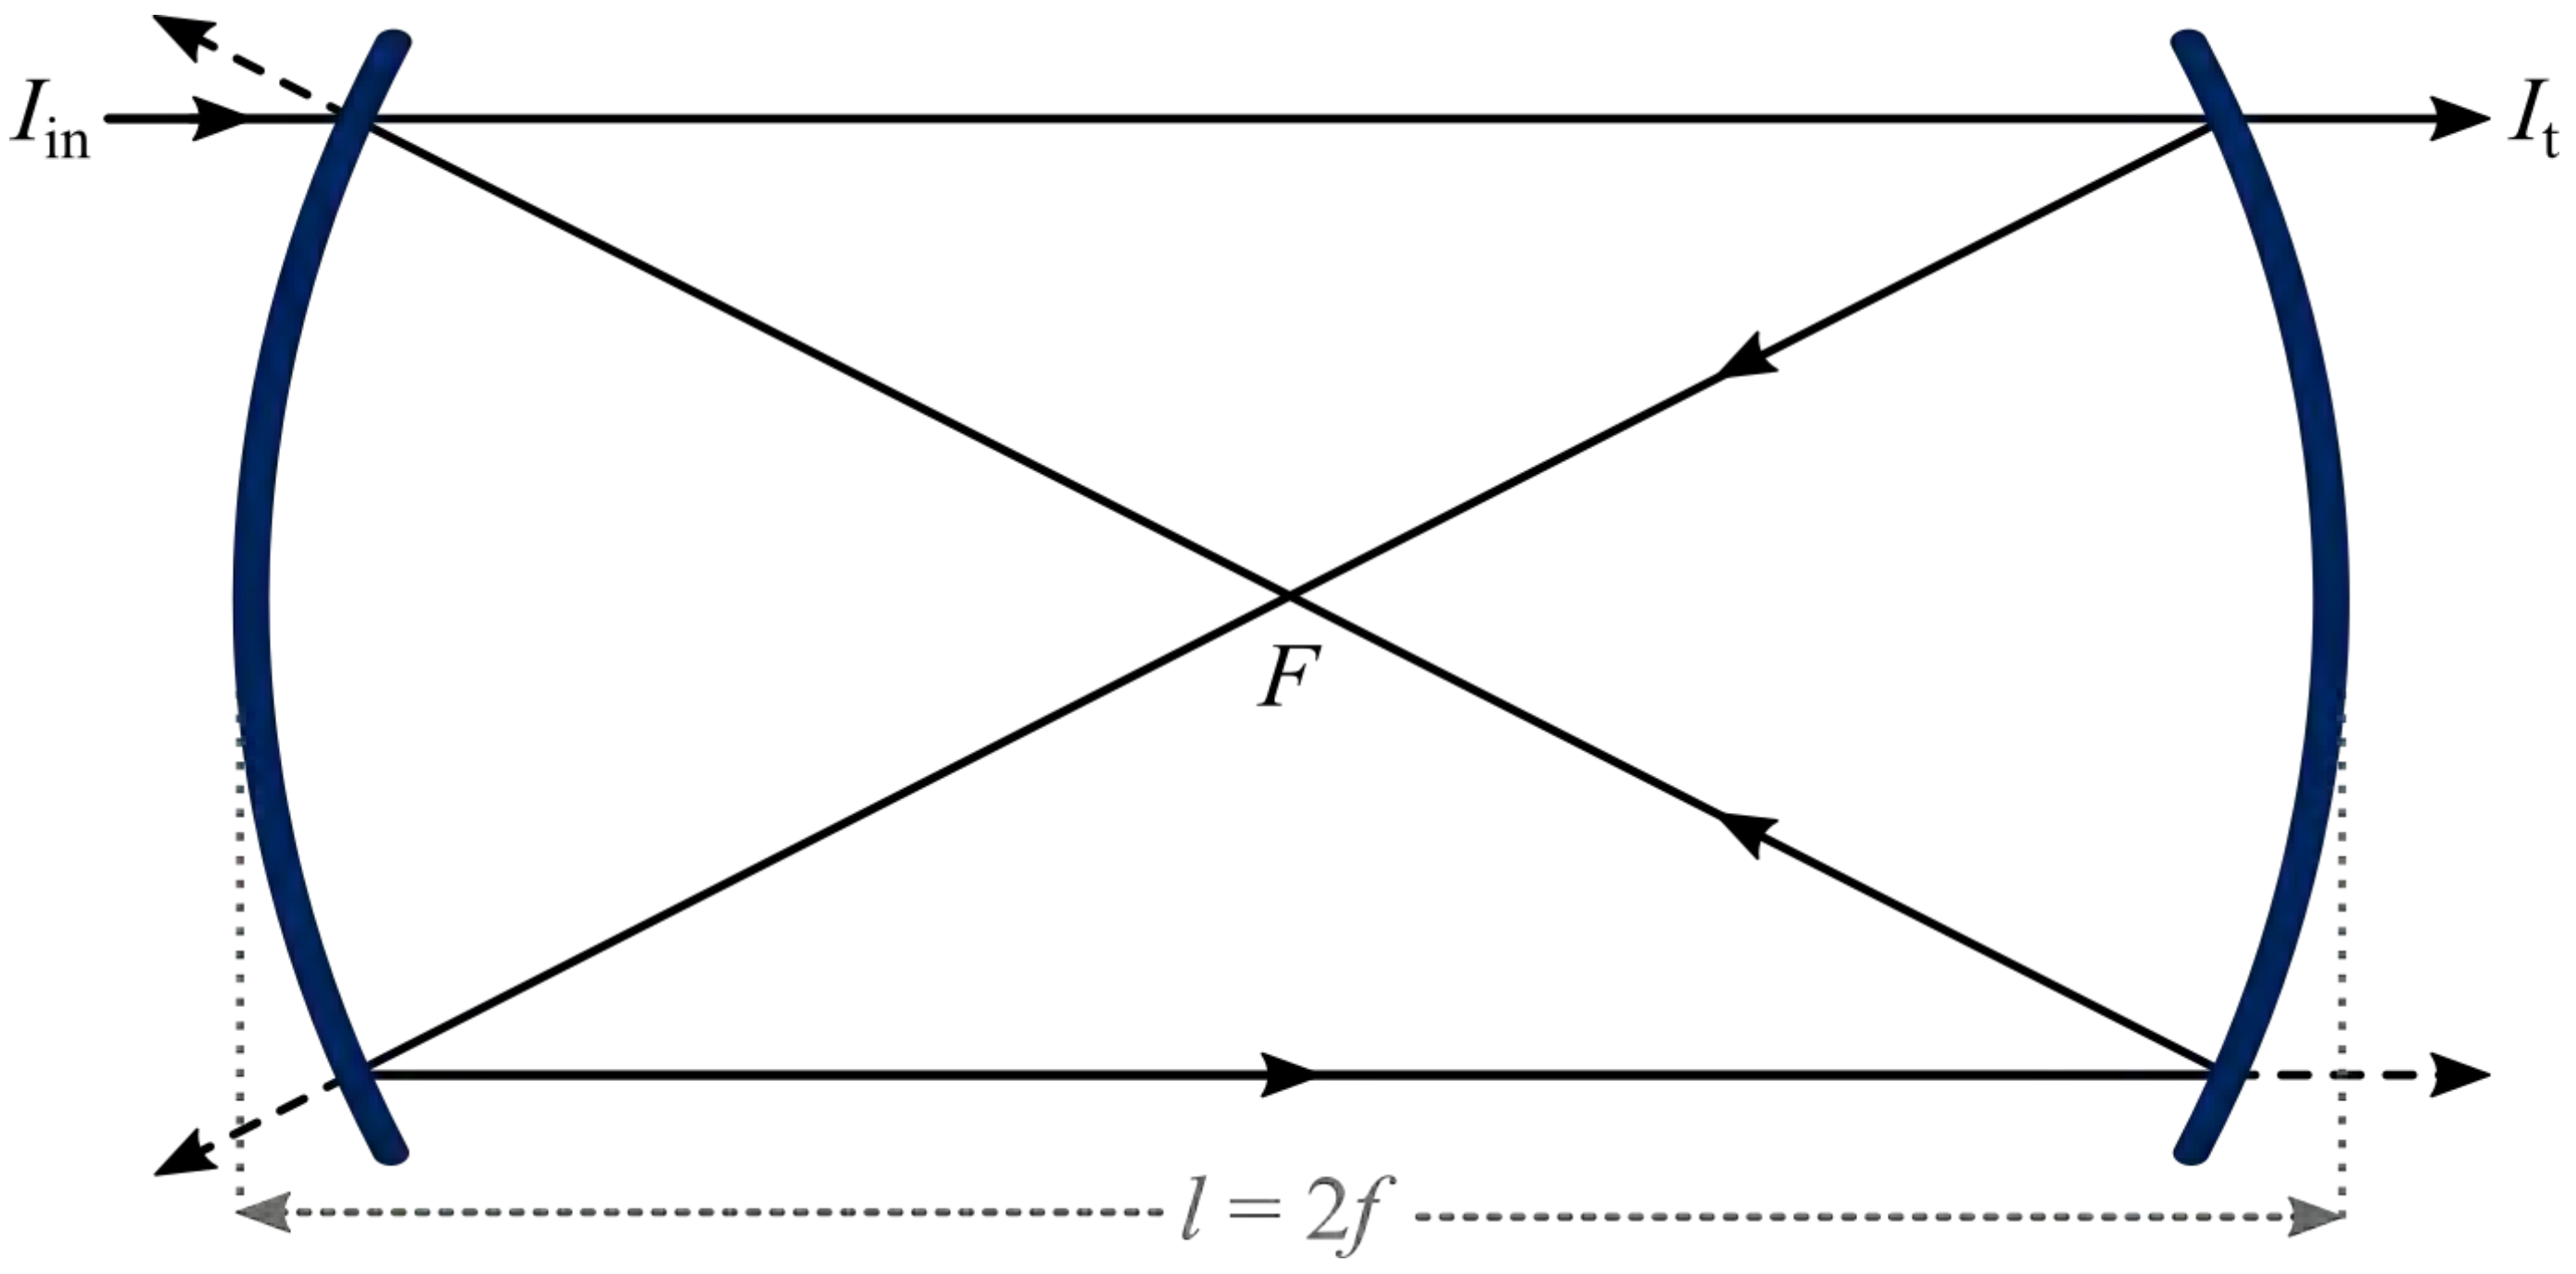
\includegraphics[width=10cm]{Confres.png}
    \caption{The beam path in a confocal resonator.}
    \label{fig:Confres.}
\end{figure}

We can't take advantage of a resonator without a light source. Here we use a \textbf{laser}, which is an acronym for ’Light amplification by stimulated emission of radiation’. The basic function principle for  a laser is the following: Inside we have a laser medium, which contains the atoms or molecules, that we can excite. That's the task of the energy pump to the extent that we get a population inversion. Now the majority of the particles are excited and absorption is dominated by stimulated emission. That means that we get more and more photons, so in other words: lights is amplified. This effect can be increased, as the laser medium is located inside of a resonator. The result is strong output radiation, which is coherent over a certain distance, monochromatic, collimated, and polarized.

The frequency range that is needed to access the $D_{2}$ transition of our rubidium atoms lies in the infrared region. For that purpose \textbf{semiconductor lasers} are generally utilized. Let's find out how the above explained function principle is applied in this case. Picking up the band structure representation for this description is the most sensible approach (see figure \ref{fig:Semiconlas.}). i) Initially there is a p-type and a n-type semiconductor with their respective Fermi energy $E^{p}_{F}$ and $E^{n}_{F}$ and their energy gap $E_{G}$. ii) After creating the p-n junction the charge concentrations are equalized through exchange of free charge carriers. This takes place until the resulting voltage compensates the diffusion voltage. The system reacts with a shift of both chemical potentials so there is only one Fermi energy $E_{F}$ and the band structure gets deformed accordingly. At the end the p side is charged positively, the n side negatively and in between is the depletion region, marked in blue. iii) If now an external voltage is applied in forward bias, then more charges accumulate in the depletion region and the Fermi energies shift against one another. Electrons in the conduction band can now move to the valence band and photons of energy $E_{G}$ are sent out. iv) So all in all the semiconductor materials serve as laser medium, the applied voltage represents the energy pump and for the right constellation of refractive indices of the semiconductor and the surrounding material the plane end faces of the semiconductor play the role of a resonator. Although the injection current $I_{in}$ needs to reach at least the threshold current $I_{th}$ for a necessary population inversion to occur.

\begin{figure}[h]
    \centering
    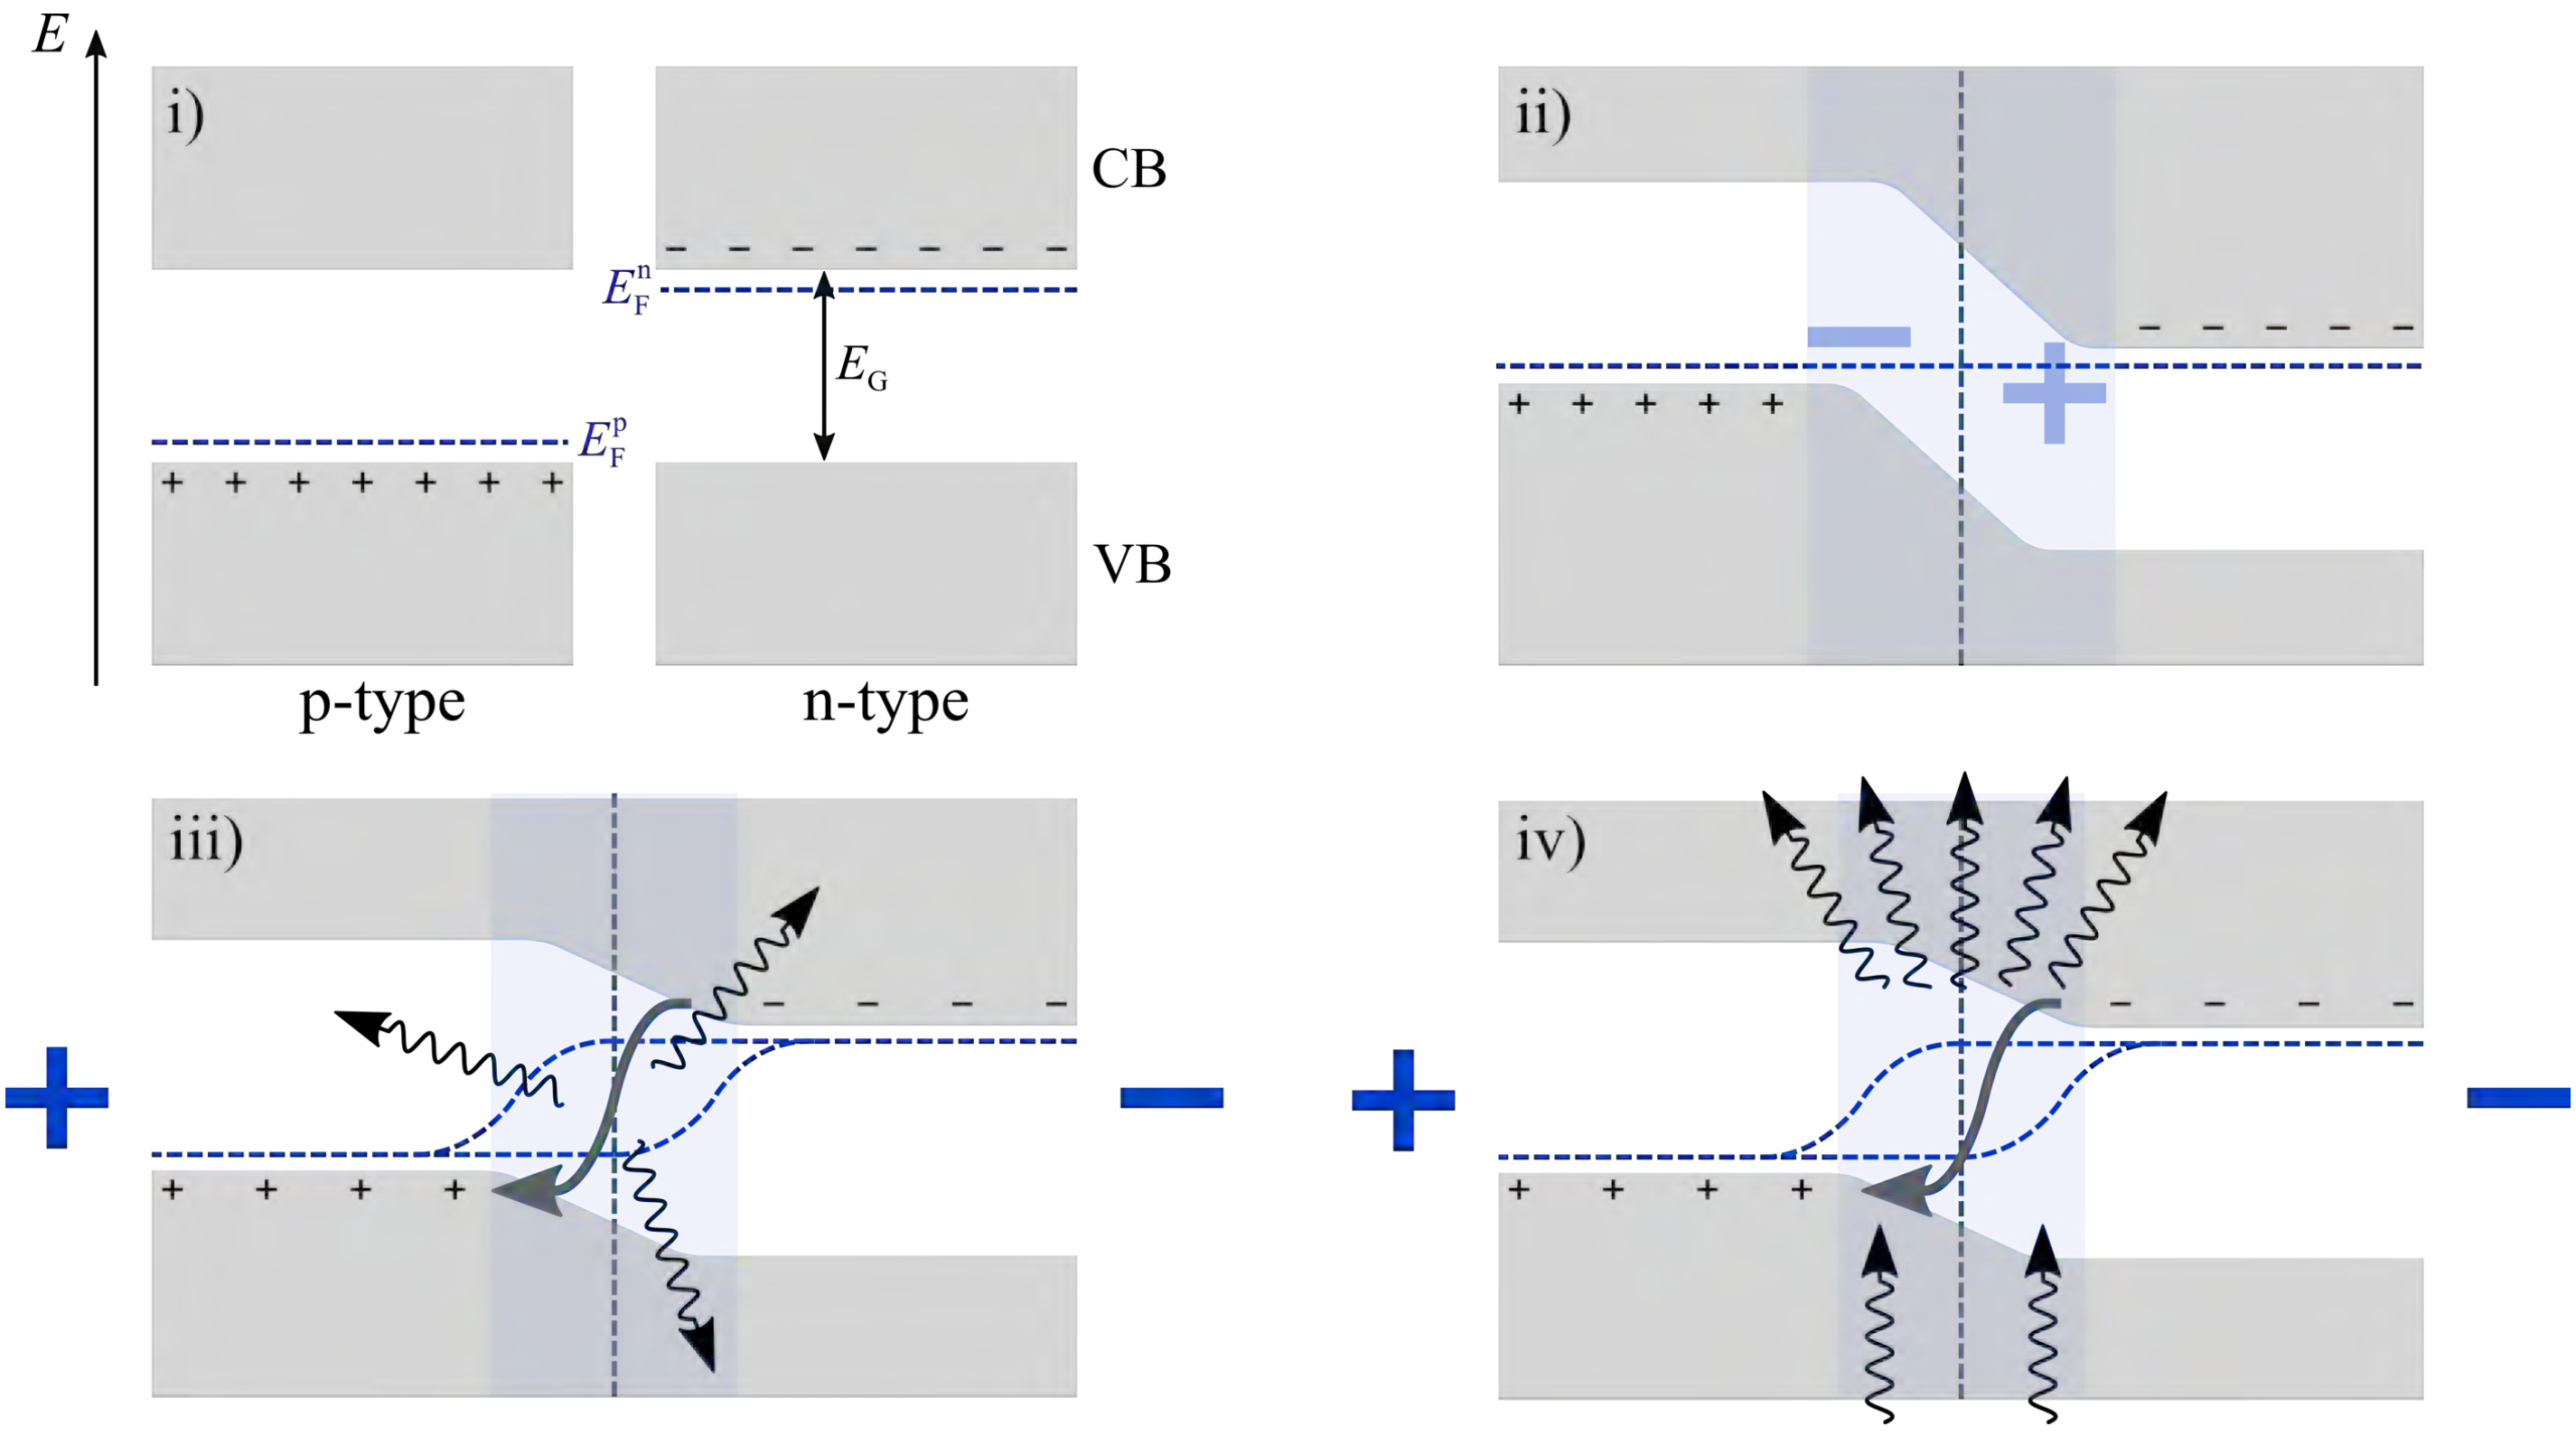
\includegraphics[width=15.8cm]{Semiconlas.png}
    \caption{The beam path in a confocal resonator.}
    \label{fig:Semiconlas.}
\end{figure}

In many aspects semiconductor lasers are advantageous but one major disadvantage is the large spectral linewidth of the resonator because of the small $l\lesssim mm$ according to equation \ref{E:speclinwid}. The solution is an additional external resonator which makes the whole apparatus to a so called \textbf{external cavity diode laser} (ECDL). An example is depicted in figure \ref{fig:ECDL}. The Littrow lattice has the purpose to enhance the free spectral range and thus achieve a single-mode operation. One part of the laser light is reflected according to Snell's law and the other part is reflected back. So the output coupler of the laser diode has to be also a good input coupler.

\begin{figure}[h]
    \centering
    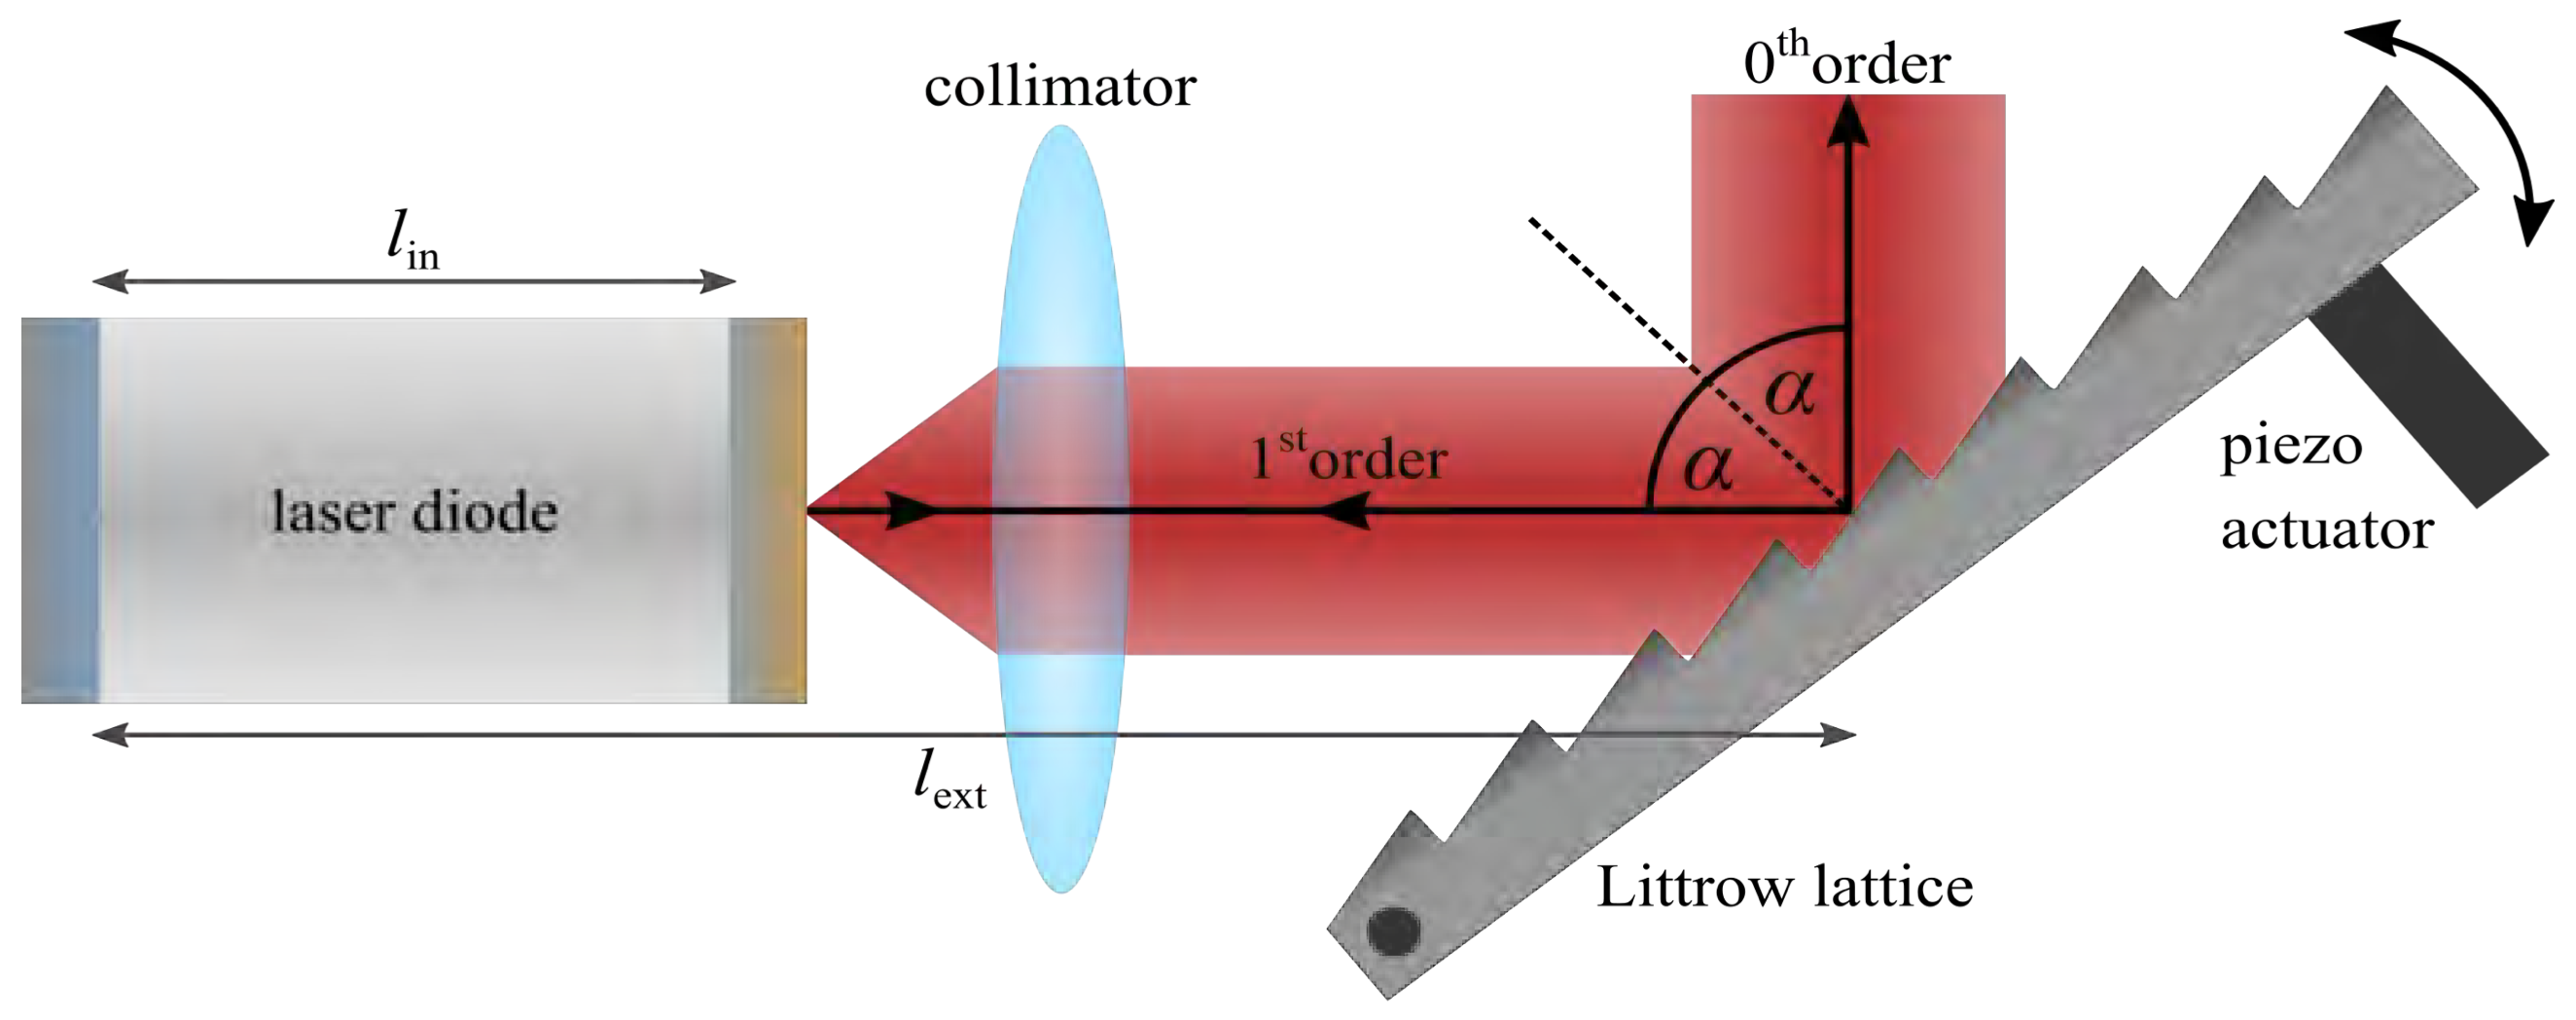
\includegraphics[width=11cm]{ECDL.png}
    \caption{A tunable ECDL in Littrow configuration.}
    \label{fig:ECDL}
\end{figure}

Lastly in this theory part it's going to be described, how the two different spectroscopy methods, used in this experiment, work. Absorption spectroscopy is in principle very simple: We change the frequency of the light permanently and measure the transmitted intenstiy with a photodiode. Saturation spectroscopy is a little more complicated with the advantage, that it's Doppler-free. This is very useful, as the Doppler broadening prevents us from seeing all the hyper fine lines in the absorption spectroscopy. The way it's done is the following: There a two overlapping beams of same wavelength but opposite direction. One is the strong pump beam and the other the weak probe beam, whereas only the intensity of the probe beam is detected. Because of the Doppler effect, just in the case of particles with velocity $v_{z}=0$ both beams are absorbed. As the pump beam has a much higher intensity, it saturates the given transition. Hence the probe beam can't be absorbed and we get a so called \textbf{Lamb-dip} in the spectrum. This is visually shown in figure \ref{fig:Lamb}.

\begin{figure}[h]
    \centering
    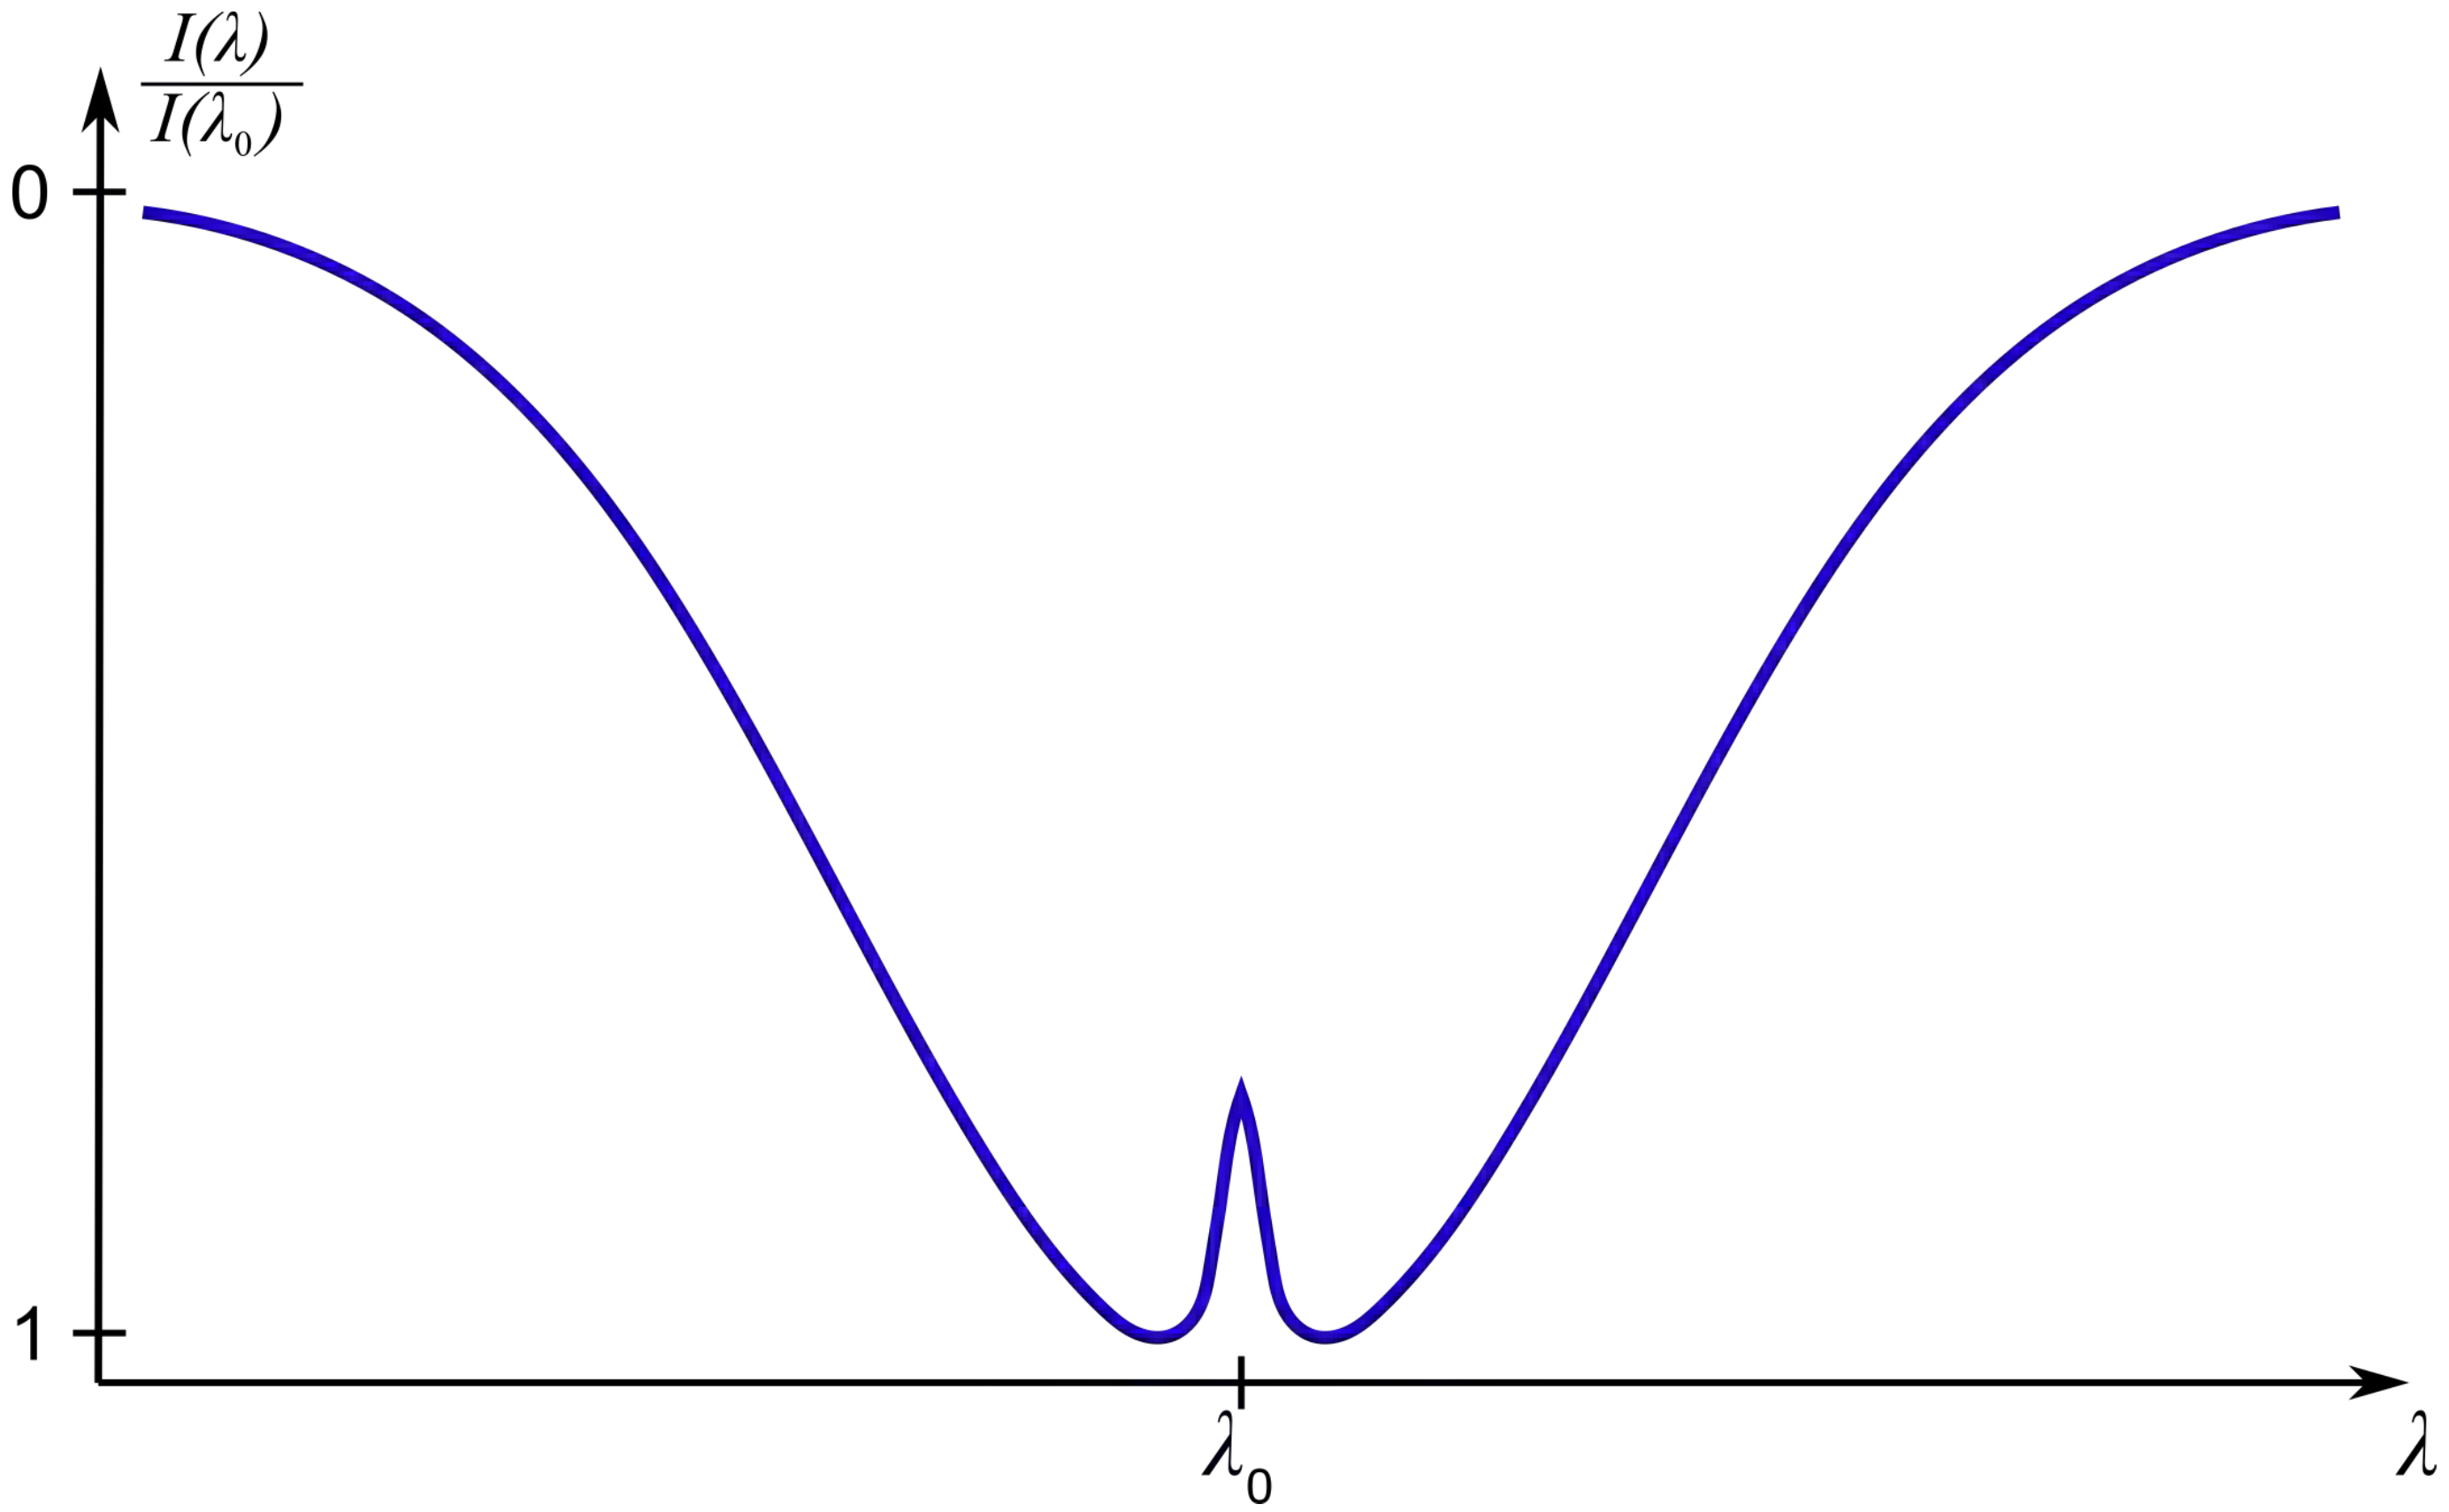
\includegraphics[width=9cm]{Lamb.png}
    \caption{Doppler-broadened absorption spectrum with a Lamb-dip at $\lambda_{0}$.}
    \label{fig:Lamb}
\end{figure}

\chapter{Experimental setup}

\begin{figure}[h]
    \centering
    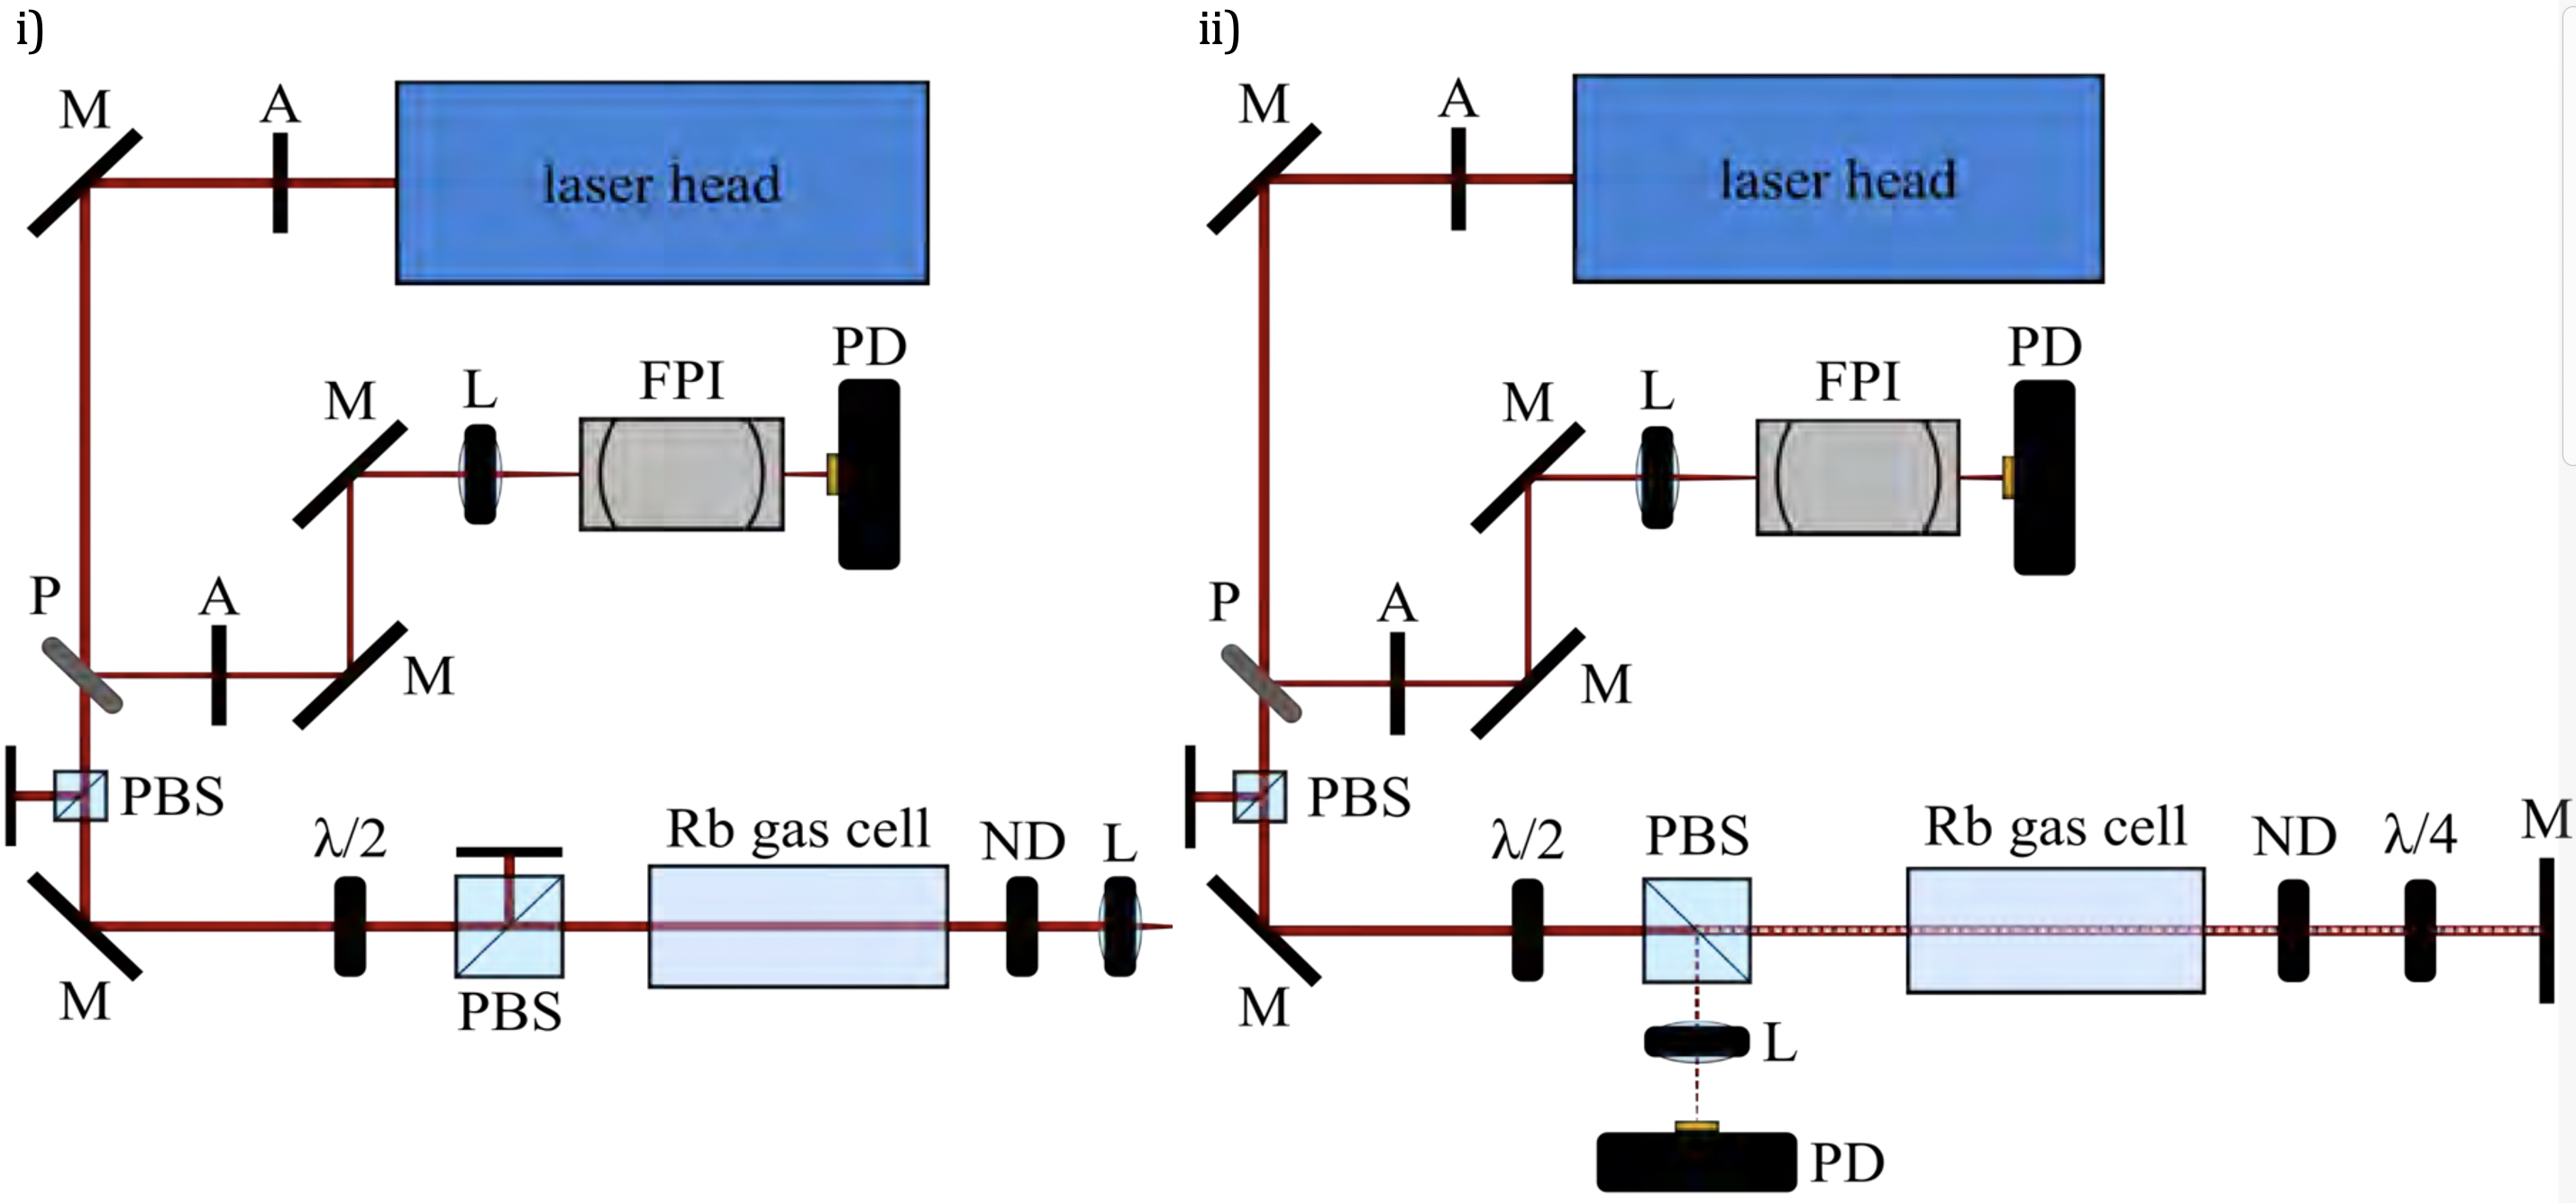
\includegraphics[width=15.8cm]{Expset.png}
    \caption{Experimental setup for i) absorption spectroscopy and ii) saturation spectroscopy.\\ A: aperture, M: mirror, P: platelet, L: lens, FPI: Fabry-Pérot interferometer, PBS: polarizing beam splitter, ND: neutral density filter, PD: photodiode}
    \label{fig:Expset}
\end{figure}

\noindent
A sketch of the experimental setup is given by figure \ref{fig:Expset}. Concerning the photodiode it has to be kept in mind, that in order to measure the intensity changes properly, the photo current should never saturate. The ND-filers are there to weaken the laser beam. That is needed, since diverse complications come along with change of the intensity directly at the laser. Every ND-filter has a value for their optical density OD, which occurs in the Beer-Lambert law $I_{t}=T\times I_{0}=10^{-OD}\times I_{0}$. To alter the polarization of the beam retarder waveplates are utilized. In the experiment we have half-wave plates ($\lambda/2$) and quarter-wave plates ($\lambda/4$). $\lambda/2$-retarder cause a phase shift of $\phi=\pi$. Also linearly polarized light can be shifted by rotating the retarder plate. $\lambda/4$-retarder cause a phase shift of $\phi=\pi/2$. So linearly polarized light is transformed into circularly polarized light and the other way around. The platelet as well as the polarizing beam splitter split the incoming beam into two beams with different directions. Just that the quartz platelet reflects only a little light and the PBS splits light of horizontal and vertical polarization. Operation of the laser is possible through the laser controller. It consists of four modules: The monitor unit DC 110, the current control unit DCC 110, the temperature control unit DTC 110 and the scan control unit SC 110. One has to be cautious while starting and stoping the laser, as there is a certain order of actions to take to do this correctly. Also the general alignment and adjustment rules have to be followed, to make sure to protect oneself and the devices from any damage. 

\chapter{Experiment execution}

Firstly the configuration as shown in figure \ref{fig:Expset} has to be set up. The ND-filter for the recording of the absorption spectrum has to have an $OD\geq 3.0$. The injection current needs to be zero at the beginning and the power supply of the PD needs to be plugged in. Before the recording of a spectrum the lasing threshold hast to be determined. Thereto increase $I_{in}$ slowly until a signal on the monitor of the oscilloscope can be seen. After that make adjustments on the oscilloscope, so the signal can be seen properly. 

Now the absorption spectrum can be recorded. At the start the focus is on the FPI signal. Set $I_{in} \approx 45mA$. and the amplitude of the SC 110 to approximately 6.5. After that set the oscilloscope trigger on the trigger signal of the SC 110. The frequency range should be set to 4. There might be again adjustments of the oscilloscope settings needed. From now on, detect in addition the signal of the Rb gas cell. For that rotate the $\lambda/2$-retarder until the signal appears on your oscilloscope display. Adjustments to the injection current, the offset and on the oscilloscope allow you to get broad dips in your spectrum. Lastly don't forget to save the image and the corresponding waveform data. Subsequently to record the saturation spectrum, the setup has again to be altered. This time a ND-filter with $OD\approx1.6$ is appropriate. Here the overlap of the pump and probe beam additionally has to be checked. Make analogous adjustments to the ones in the first experimental task until you get a favorable spectrum. Again save the data for the evaluation. 

    \chapter{Analysis of the Data}
    \section{The Data}
The data for this experiment was Taken via the CSV function of a four channel oscilloscope. It is connected to photo-diodes behind the farby-perot
interferometer (CH2), a trigger signal from the laser (CH1) and one photo diode behind the rubidium cell (CH3).

Due to a name collision while transferring the data from the USB-stick that was written to by the oscilloscope to the Computer, the data of the First
part was overwritten and subsequently lost. An attempt is made to reconstruct the information of the first Part by adequately masking the data that
was gathered and survived the transfer to the computer.

The oscilloscope was set to record 20,000,000 samples. This data was first condensed via the calculation of the Mean value for all channels within an
interval of $4\cdot 10^{-6} \text{[s]}$ and working with that data. Due to this reduction of data, a proper standard deviation could be calculated for
every data point in the reduced data set.

The Same slope was again taken in higher time resolution in a second measurement, also set to record 20,000,000 measurements.

\begin{figure}[tb]
	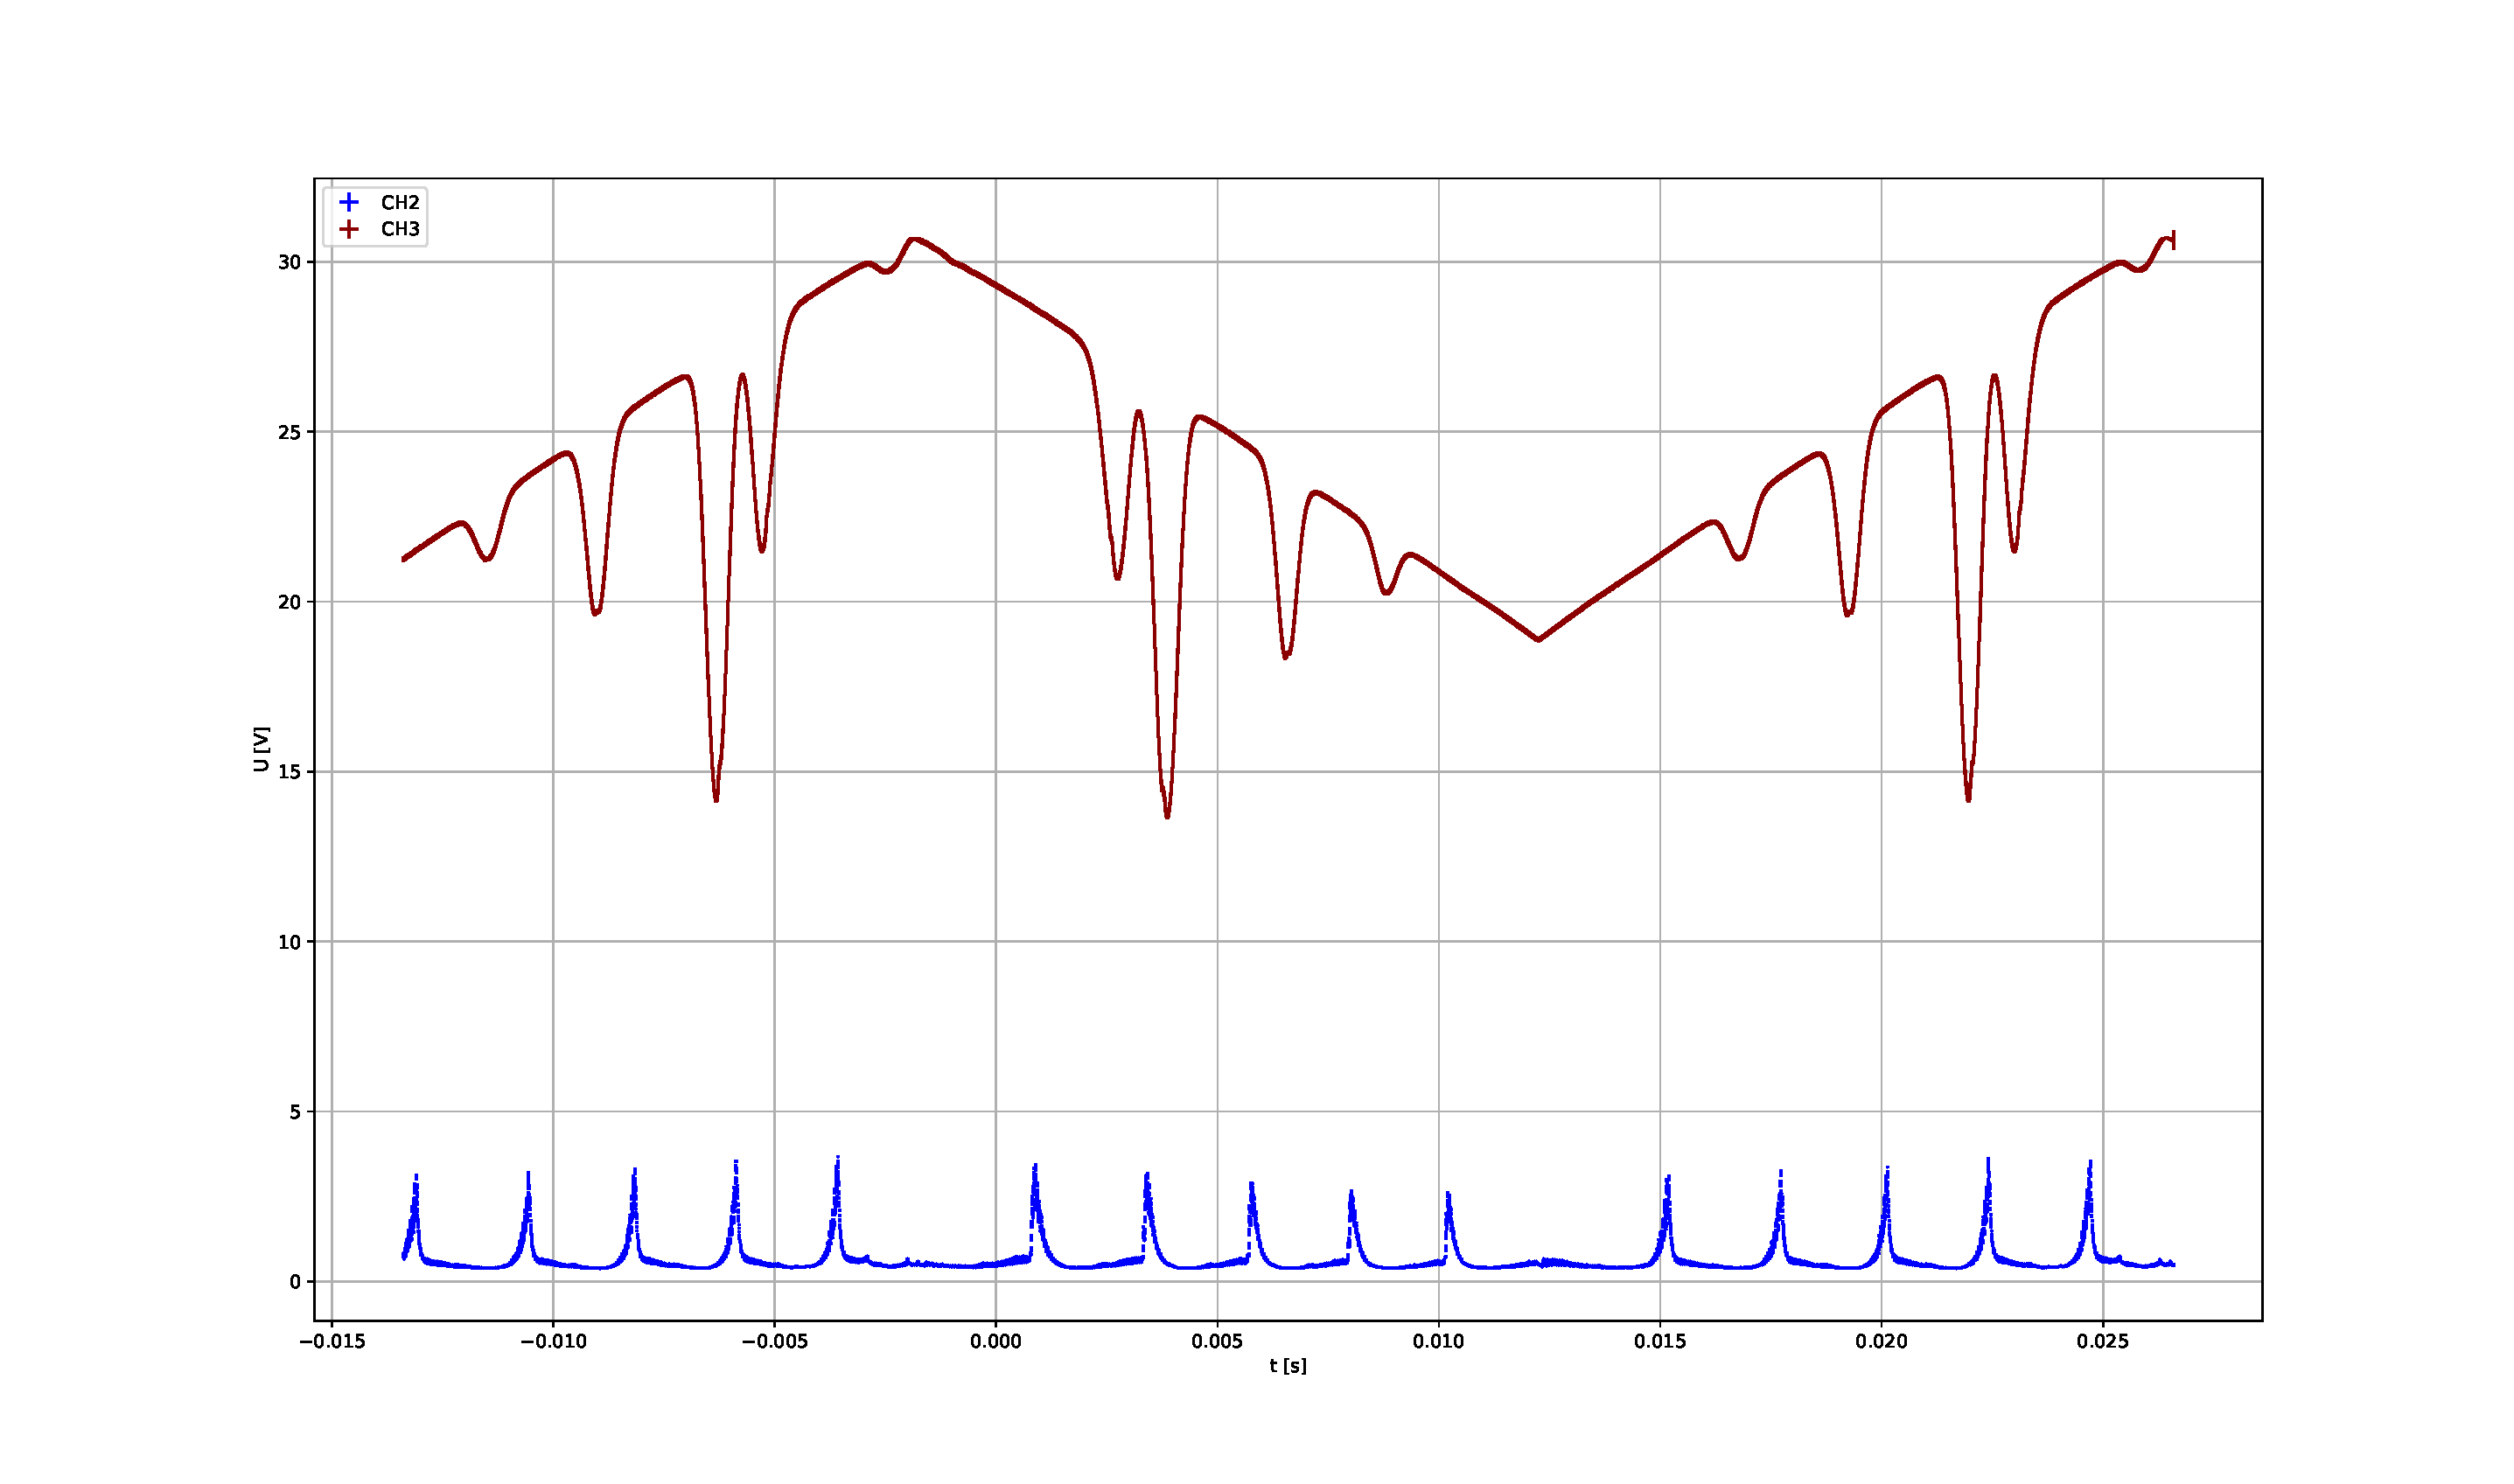
\includegraphics[width=\textwidth]{fig/data_overview_large.pdf}
	\caption{The averaged data for the Channels 2 and 3 as they contain the information of interest}
	\label{fig:data_overview_large}
\end{figure}

\begin{figure}[tb]
	\includegraphics[width=\textwidth]{fig/data_overview_small.pdf}
	\caption{The averaged data for the Channels 2 and 3 as they contain the information of interest. This is the Measurement with a higher time
	resolution}
	\label{fig:data_overview_small}
\end{figure}

\subsection{Splitting the large Dataset}
To increase the amount of usable Data, the large dataset is split into three smaller sets, that are mirrored and shifted as to fit to the other data.
To find the cut points, the maximum and minimum values of the background slope are used as cutting points. After this step every dataset is treated
identically.

\section{Determining the Conversion factor from time to frequency}
As the quantity of interest is the frequency and not the Time of the measurement relative to the trigger, the time needs to be converted into a
relative frequency. This is done using the resonance peaks of the farby-perot interferometer on channel 2. These peaks are $2.5 \text{[GHz]}$ apart,
and serve as frequency markers. With these it is possible to calculate a conversion factor.

To determine their distance in time, the peaks are first fitted to lorentz resonance functions of the form:
$$ f(\omega) = \frac{1}{(\omega^2-\omega_0^2)^2 + \gamma^2\omega_0^2}$$

To fit the individual peaks, the dataset is cut into adjacent regions, each containing one peak. The result of the fits 

\begin{figure}[tb]
	\includegraphics[width=\textwidth]{fig/fitted_spikes_ramp_0.pdf}
	\caption{The peaks on Channel 2 fitted to lorentz functions for the first dataset}
	\label{fig:data_overview_small}
\end{figure}

\begin{table}
	\begin{center}
		\label{tab:freq_peaks}
		\begin{tabular}{|m{10em} m{10em} m{10em}|}
			\hline
			\textbf{Peak/Dataset No.} & Peak time [s] & $\textbf{FWHM}/2$ [s] \\
			\hline\hline
			1/1 & 0.00260 & 0.00008 \\
			1/2 & 0.00190 & 0.00010 \\
			1/3 & 0.00192 & 0.00008 \\
			1/4 & 0.00261 & 0.00008 \\
			\hline
			2/1 & 0.00490 & 0.00008 \\
			2/2 & 0.00444 & 0.00010 \\
			2/3 & 0.00420 & 0.00008 \\
			2/4 & 0.00488 & 0.00008 \\
			\hline
			3/1 & 0.00718 & 0.00008 \\
			3/2 & 0.00680 & 0.00009 \\
			3/3 & 0.00650 & 0.00008 \\
			3/4 & 0.00718 & 0.00008 \\
			\hline
			1/4 & 0.00957 & 0.00008 \\
			2/4 & 0.00906 & 0.00009 \\
			3/4 & 0.00888 & 0.00009 \\
			4/4 & 0.00957 & 0.00008 \\
			\hline
		\end{tabular}
		\caption{The location and width of the Farby-Perot interferometer resonance peaks}
	\end{center}
\end{table}

The peaks from every dataset are listed in the table \ref{tab:freq_peaks}. For the peaks the full width at half max was used to judge the accuracy of
the measured peak. From this the distance between the peaks was measured and multiplied with the distance of the peaks in frequency due to the
knowledge of the Farby-Perot interferometer. The distance of the resonances of the farby perot interferometer is estimated to be: $\delta f = 2.500
\pm 0.001 \text{GHz}$.

For every consecutive pair of peaks the distance in time is computed from the table \ref{tab:freq_peaks}. The mean of all distances is calculated
together with it's error, which includes the errors from the peaks that was propagated into the error of the distances which is in turn propagated
into the uncertainty of the mean distance. The mean time distance of the FP-Peaks is $\Delta t = 0.00234 \pm 0.00003 \textbf{[s]}$. The conversion
factor from time to frequency is calculated from this mean and is $\frac{\Delta f}{\Delta t} =(1.069  \pm 0.014) \cdot 10^{12}
\frac{\text{[Hz]}}{\text{[s]}}$
\begin{table}
	\begin{center}
		\label{tab:freq_peaks}
		\begin{tabular}{|m{10em} m{10em} m{10em}|}
			\hline
			\textbf{Dataset No.} & a$\cdot10^{-10}\pm \sigma$  & $b \pm \sigma$ \\
			\hline\hline
			1 & $-7.826 \pm 0.004$ & $29.502 \pm 0.002$ \\
			2 & $-7.954 \pm 0.002$ & $28.6094 \pm 0.0014$ \\
			3 & $-7.884 \pm 0.002$ & $29.5240 \pm 0.0016$ \\
			4 & $-7.728 \pm 0.003$ & $29.4836 \pm 0.0006$ \\
			\hline
		\end{tabular}
		\caption{The parameters for the slopes fits of the different datasets}
	\end{center}
\end{table}
Using the Average of the distances comes at the cost of neglecting differences in the datasets which are slight, but present. The largest problem is
dataset 2 which is the falling slope of the large measurement see figure \ref{fig:data_overview_large}. The distances of it's peaks decreases towards
the end of the dataset, causing noticeable errors. This dataset also contains a shift in timing that is non-uniform. It messes with the fits and the
results from this dataset are consistently worse than the others.

As the absolute frequency cannot be given, a relative frequency is used. For this a reference point is needed. The first FP-peak of every dataset is
used and the data is shifted so that the peak is at $f = 0$.

Now that the conversion factor is known the time is converted to the frequency and the corresponding errors propagated. The result can be seen in
figure \ref{fig:frequency_conversion}.
\begin{figure}[tb]
	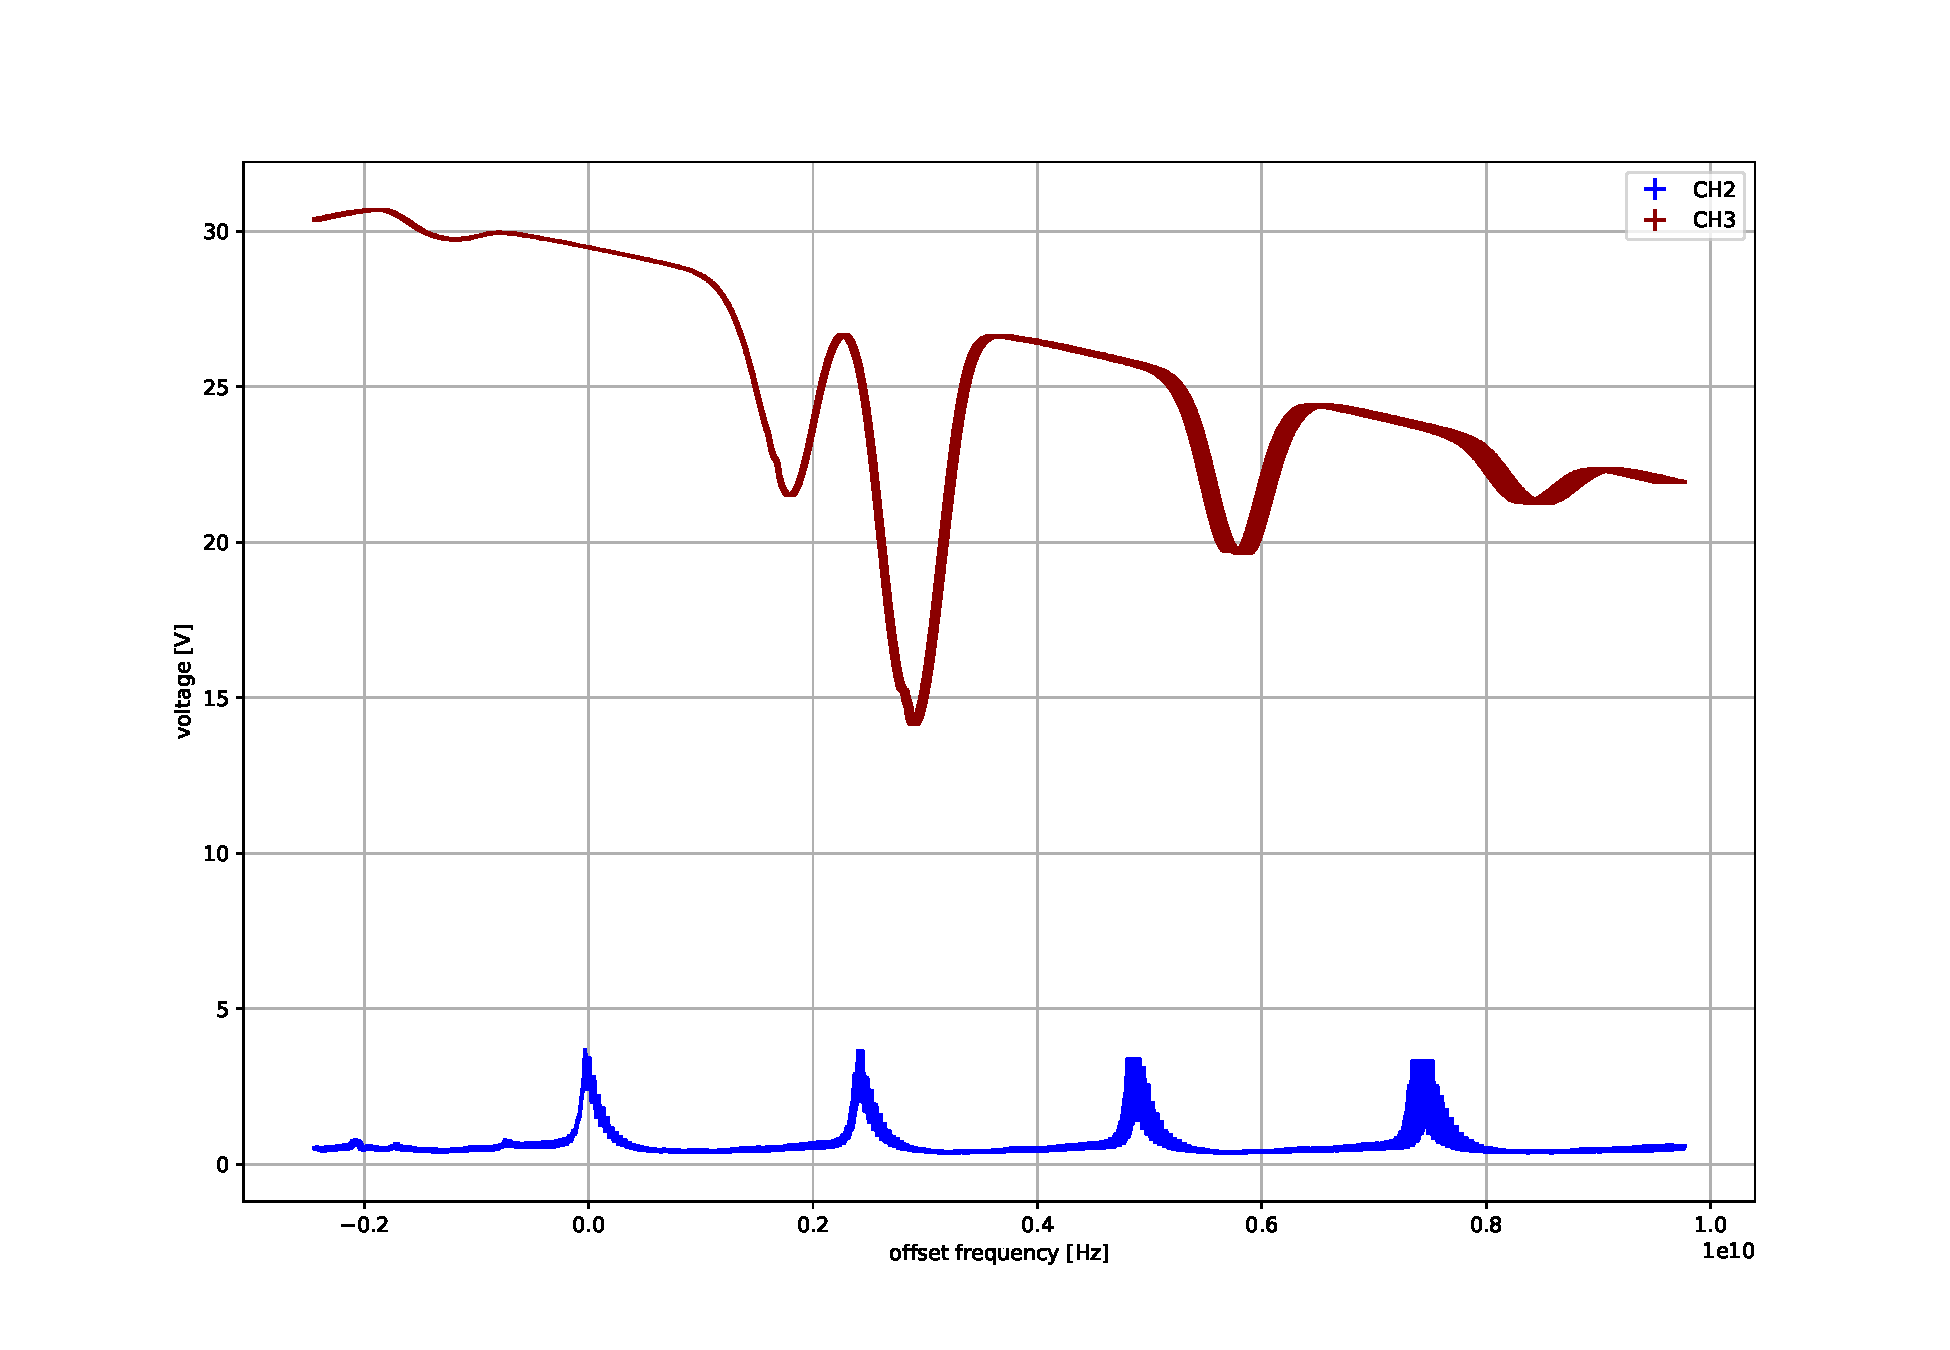
\includegraphics[width=\textwidth]{fig/ramp_3_with_error_propagation.pdf}
	\caption{The fourth (high resolution) dataset with the time converted to frequency. The uncertainties introduced by the frequency conversion are clearly
	noticeable}
	\label{fig:frequency_conversion}
\end{figure}

\section{Fitting the background slope}
To fit the background slope, the dips in intensity need to be cut out from the data, as they would otherwise interfere. As There is uncertainty in
both the frequency and the voltage, The least squares fitting method is no longer sufficient as it expects an error free frequency measurement. To be
able to include both errors, the orthogonal distance regression method is used. As the name suggests it uses the minimal orthogonal distance from the
curve to each data point as the loss function to be minimized and uses weights to incorporate the uncertainty in both dimensions.
\begin{figure}[tb]
	\includegraphics[width=\textwidth]{fig/linear_fit_3.pdf}
	\caption{The fourth dataset with the dips from the absorption removed and a fitted linear function}
	\label{fig:slope_fit}
\end{figure}

The fit for the fourth dataset is shown in figure \ref{fig:slope_fit}. The parameters of the fit $f(x) = ax + b$ are $a = (-7.728 \pm 0.003) \cdot 10^{-10}
\text{[V/Hz]}$ and $b = (29.4836 \pm 0.0006) \text{[V]}$. The fit must be done for each dataset, as the differences between them are to to yield good
results.

The Slope is then subtracted from the data, and the corresponding fit uncertainties propagated into the Data points.
\begin{figure}[tb]
	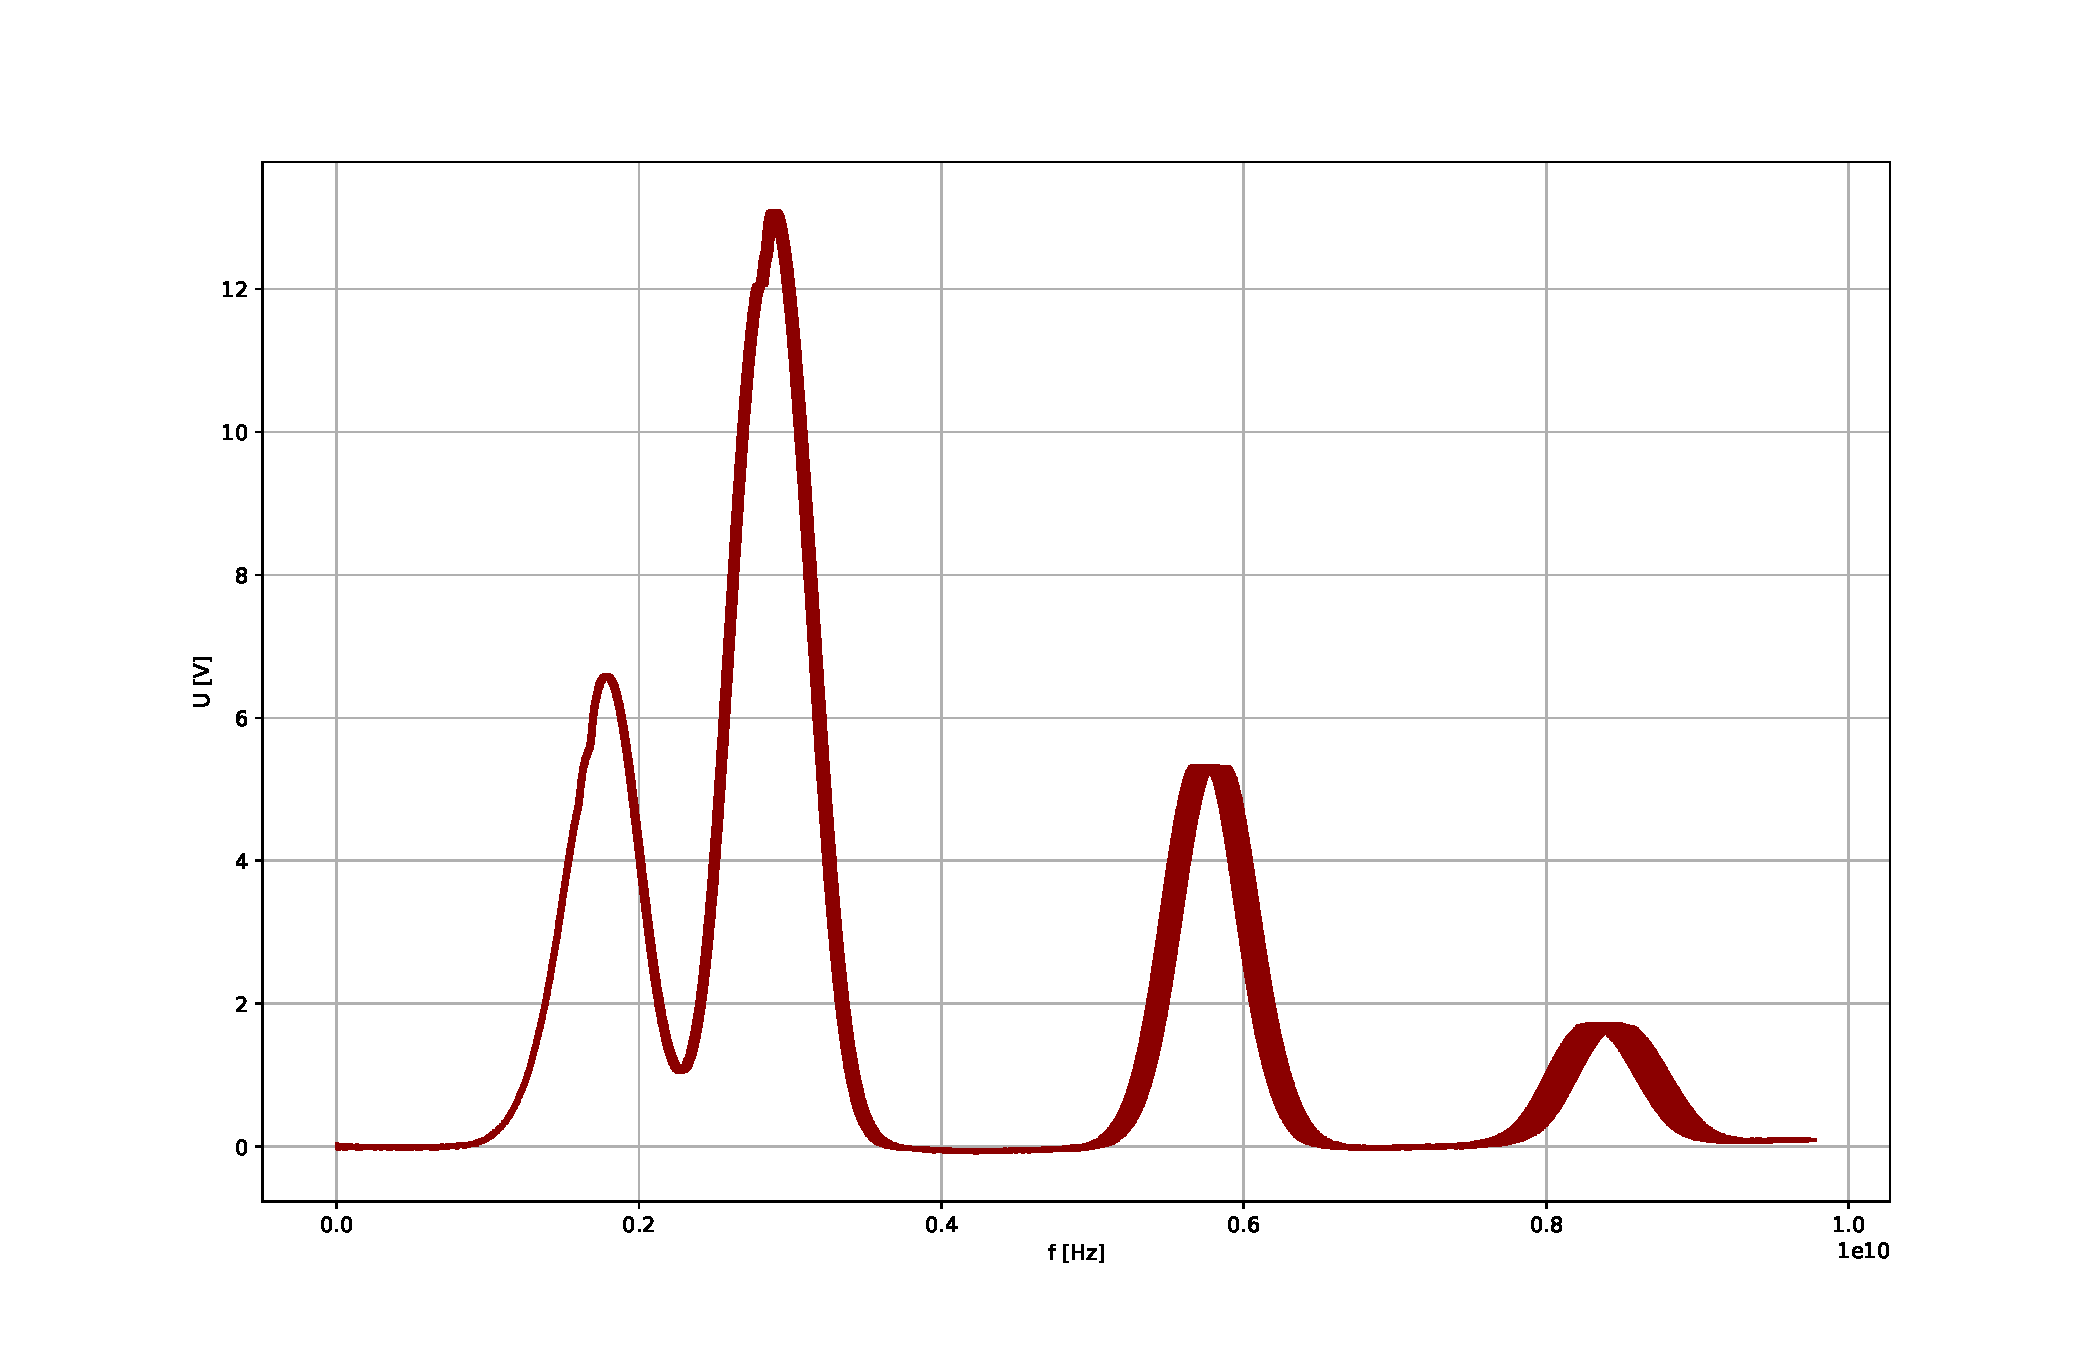
\includegraphics[width=\textwidth]{fig/data_3_without_slope.pdf}
	\caption{The fourth dataset with the background slope subtracted}
	\label{fig:data_without_slope}
\end{figure}

\section{Fitting the peaks}
With the data like in figure \ref{fig:data_without_slope} the peaks can now be fitted. For this the same orthogonal distance regression method is
used. The part of the data, that is distorted by the Saturation peaks is cut out of the data to be fitted. Similarly the peaks regions are cut out of
the rest of the data. It was chosen to fit the two close peaks separately as the fit quality was not significantly better fitting them together and
treating them separately would have meant data handling overhead. An example of the fitted data can be found in \ref{fig:fitted_peaks}

\begin{figure}[tb]
	\includegraphics[width=\textwidth]{fig/peaks_of_measurement_3.pdf}
	\caption{The fourth dataset with the peaks fitted to Gaussian curves}
	\label{fig:fitted_peaks}
\end{figure}

The fitting procedure was done for every dataset. From the location values together with their uncertainties the distances between the absorption
peaks is calculated and the distances Averaged. The corresponding uncertainties of the peak locations are again propagated into the uncertainty of the mean.

\begin{table}
	\begin{center}
		\label{tab:freq_peaks}
		\begin{tabular}{|m{10em} m{10em}|}
			\hline
			\textbf{Peak -> Peak} & $\Delta f \pm \sigma$ [GHz]\\
			\hline\hline
			1 $\->$ 2& $ 1.139 \pm 0.001$ \\
			2 $\->$ 3& $ 2.9058 \pm 0.0008$ \\
			3 $\->$ 4& $ 2.5686 \pm 0.0006$ \\
			\hline
		\end{tabular}
		\caption{The distances of the peaks}
	\end{center}
\end{table}

\subsection{Subtracting the peaks from the Data}
After fitting the peaks the expectation value can be subtracted from the data. The results are shown in figure \ref{fig:data_0_absorption} to
\ref{fig:data_3_absorption}.

\begin{figure}[tb]
	\includegraphics[width=\textwidth]{fig/Absorption_peaks_data_0.pdf}
	\caption{The first dataset with the slope and peak 'background' subtracted}
	\label{fig:data_0_absorption}
\end{figure}
\begin{figure}[tb]
	\includegraphics[width=\textwidth]{fig/Absorption_peaks_data_1.pdf}
	\caption{The second dataset with the slope and peak 'background' subtracted}
	\label{fig:data_1_absorption}
\end{figure}
\begin{figure}[tb]
	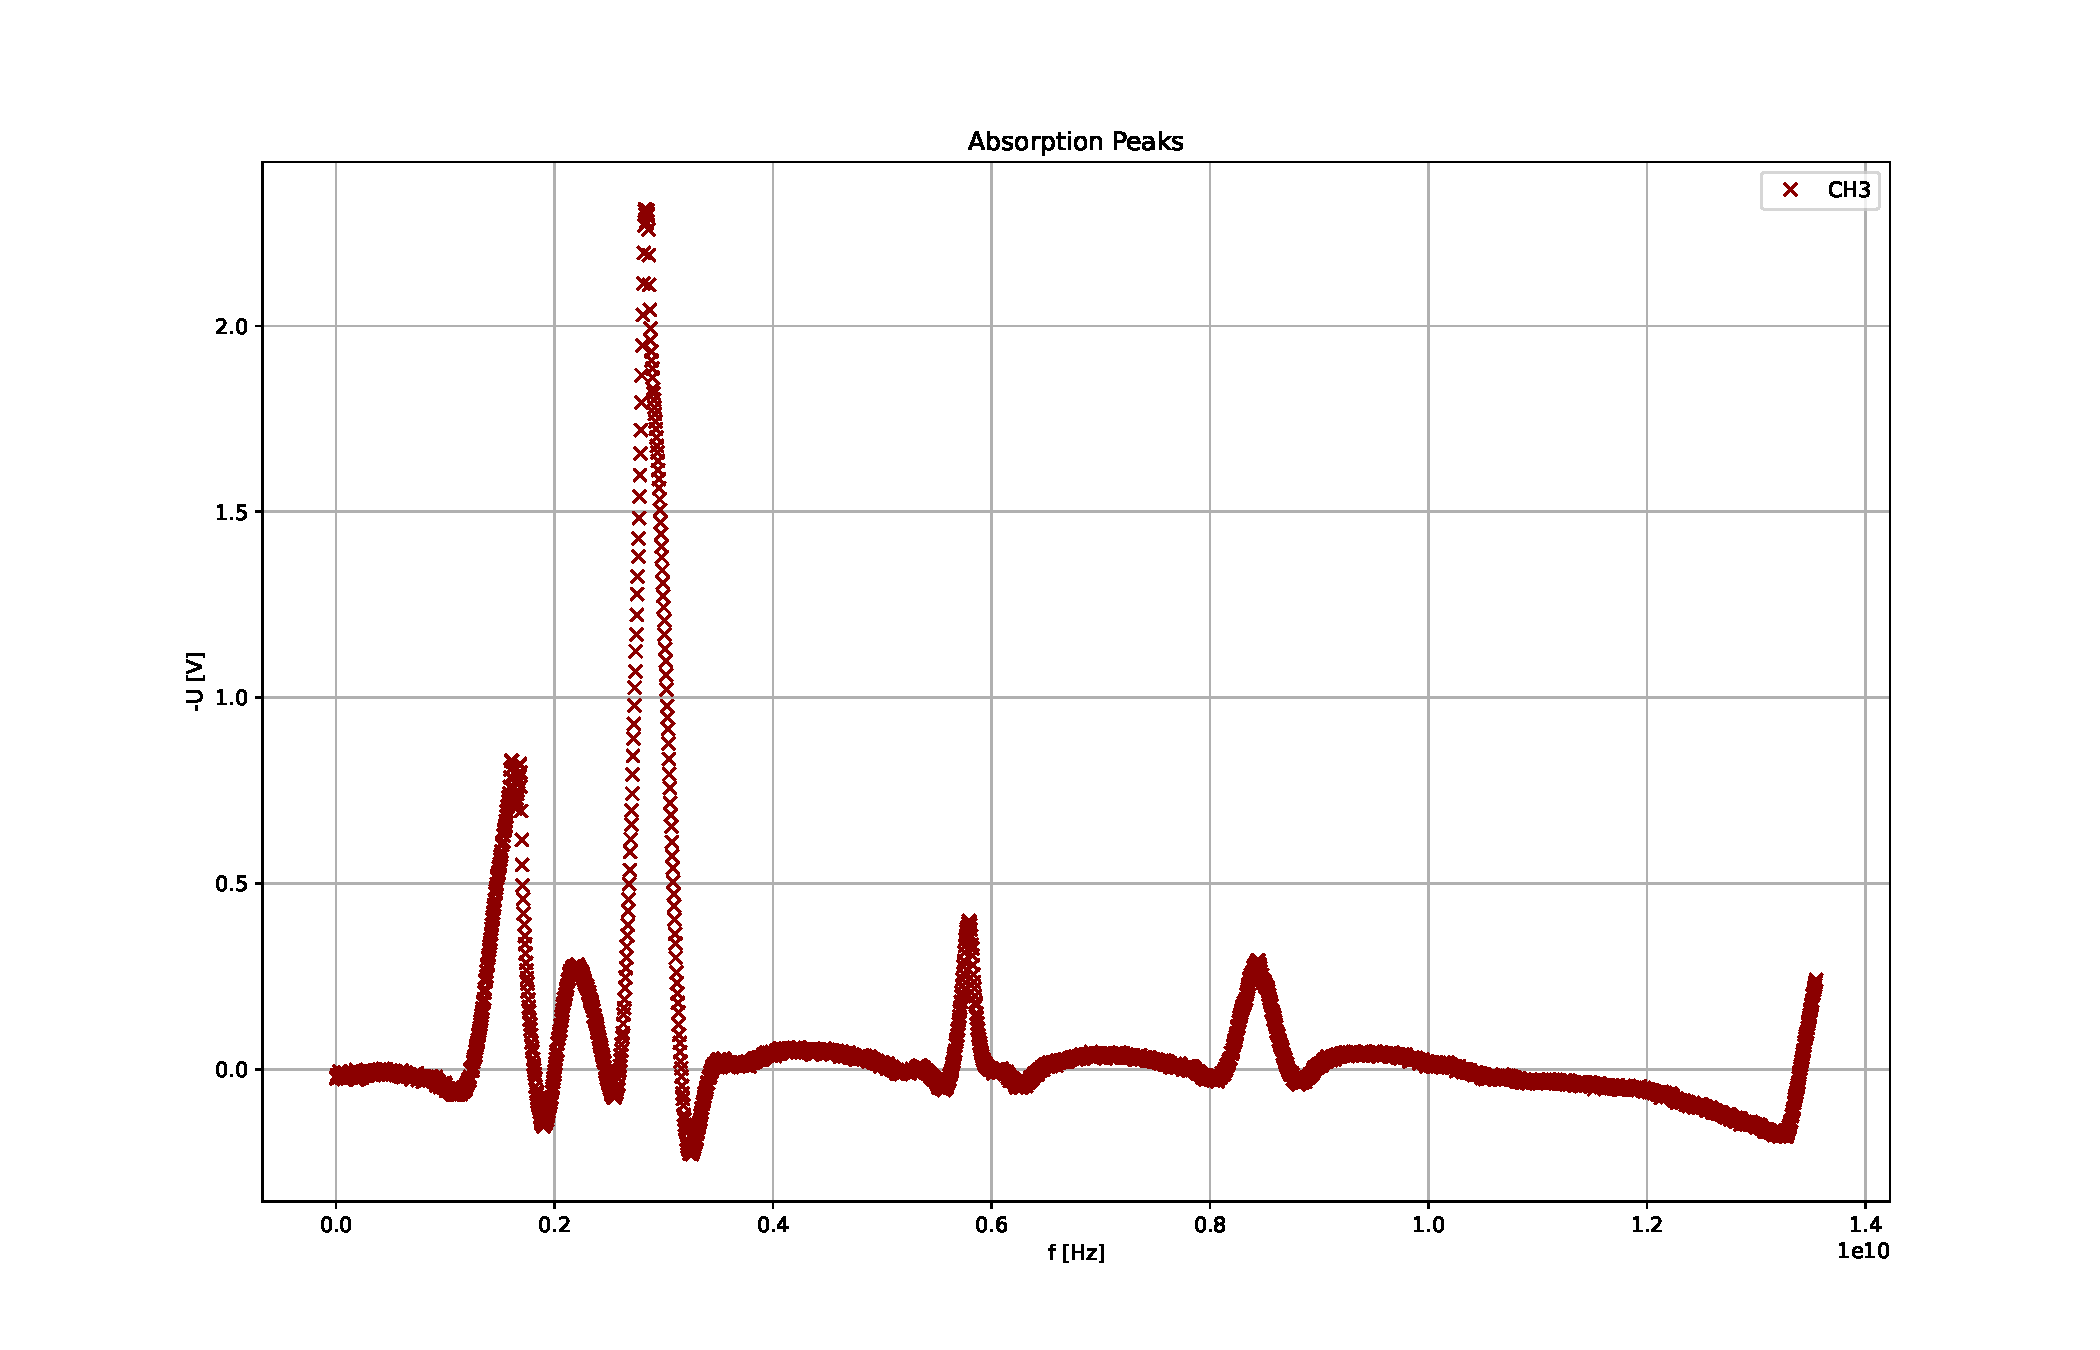
\includegraphics[width=\textwidth]{fig/Absorption_peaks_data_2.pdf}
	\caption{The third dataset with the slope and peak 'background' subtracted}
	\label{fig:data_2_absorption}
\end{figure}
\begin{figure}[tb]
	\includegraphics[width=\textwidth]{fig/Absorption_peaks_data_3.pdf}
	\caption{The fourth dataset with the slope and peak 'background' subtracted}
	\label{fig:data_3_absorption}
\end{figure}

As can be seen, the data in figure \ref{fig:data_1_absorption} was not approximated well by the fit curves. this can be seen by the large amplitude in
behind the second peak and between the first and second peak. As the quality of the data measured in the fourth dataset, the subsequent fits will only
be performed on the fourth Dataset.

The Peaks that can still be seen in \ref{fig:data_3_absorption} are not of the shape of lorenz peaks, and still contain a lot of other background.
This is probably due to the missing 'clean' data from the runs that where overwritten, as the Gaussian functions have more available points that are
not distorted by the resonance absorption, resulting in a better fit, and better background suppression.

\section{Finding the Resonance Absorption peaks}
If however the data is again cut down to the features of interest, some lorentz like peaks can be recognized.
These will be examined further.

Due to the many uncertainties that have amassed so far, doing an uncertainty estimation here is effortfull and will most likely only yield
uncertainties that are far larger than the features that are to be examined. Propagating the Error from the subtraction of the Gaussian into the
uncertainties of the points is beyond the scope of this report. So for the following there will be no uncertainty estimation.

\begin{figure}[tb]
	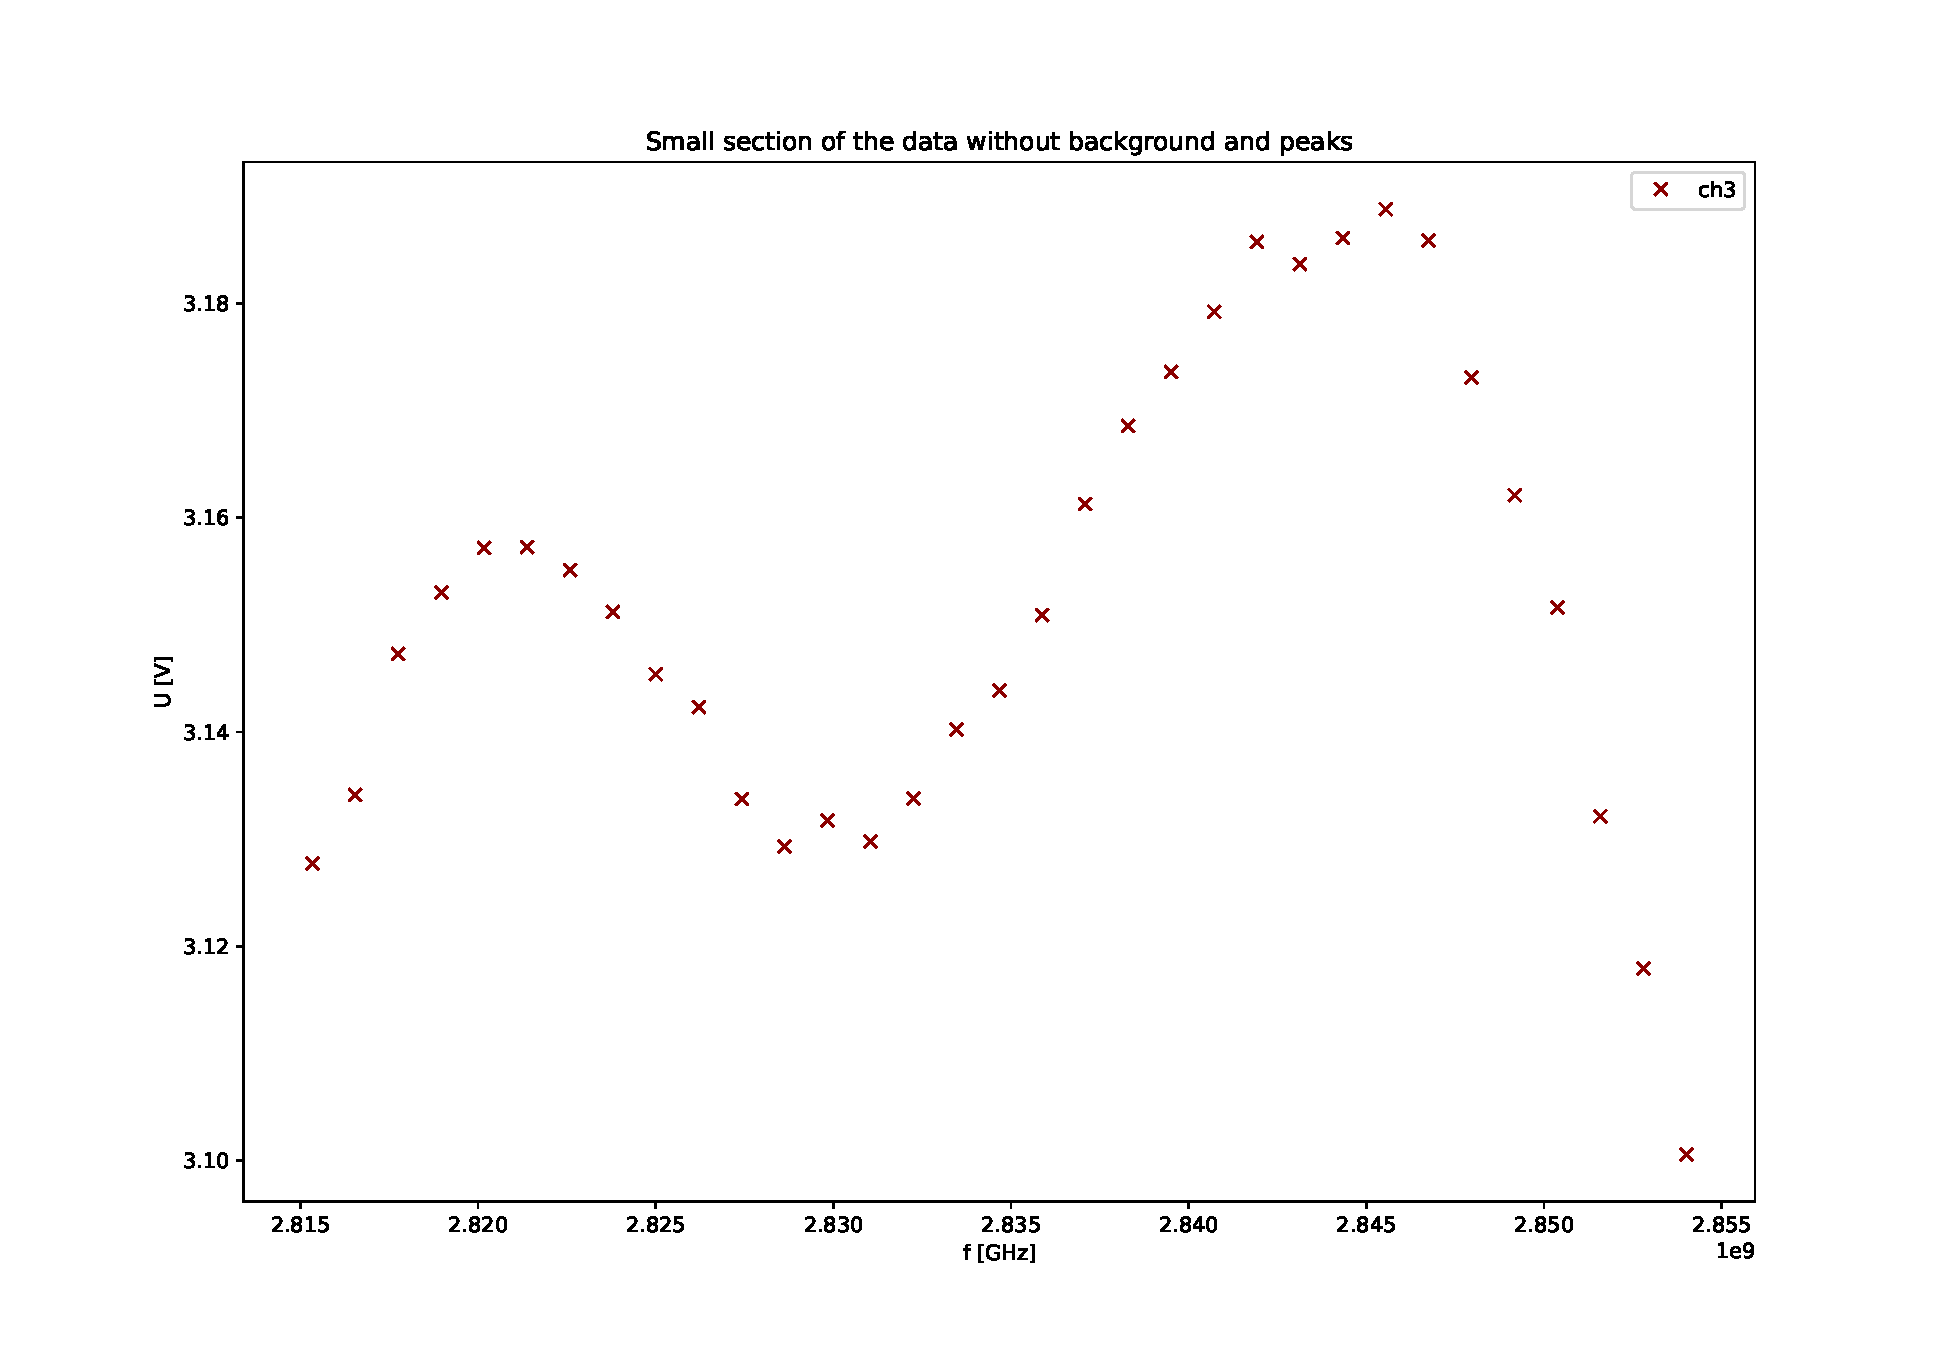
\includegraphics[width=\textwidth]{fig/absorption_cut_0.pdf}
	\caption{The first cut from the fourth dataset}
	\label{fig:absorption_cut_0}
\end{figure}
\begin{figure}[tb]
	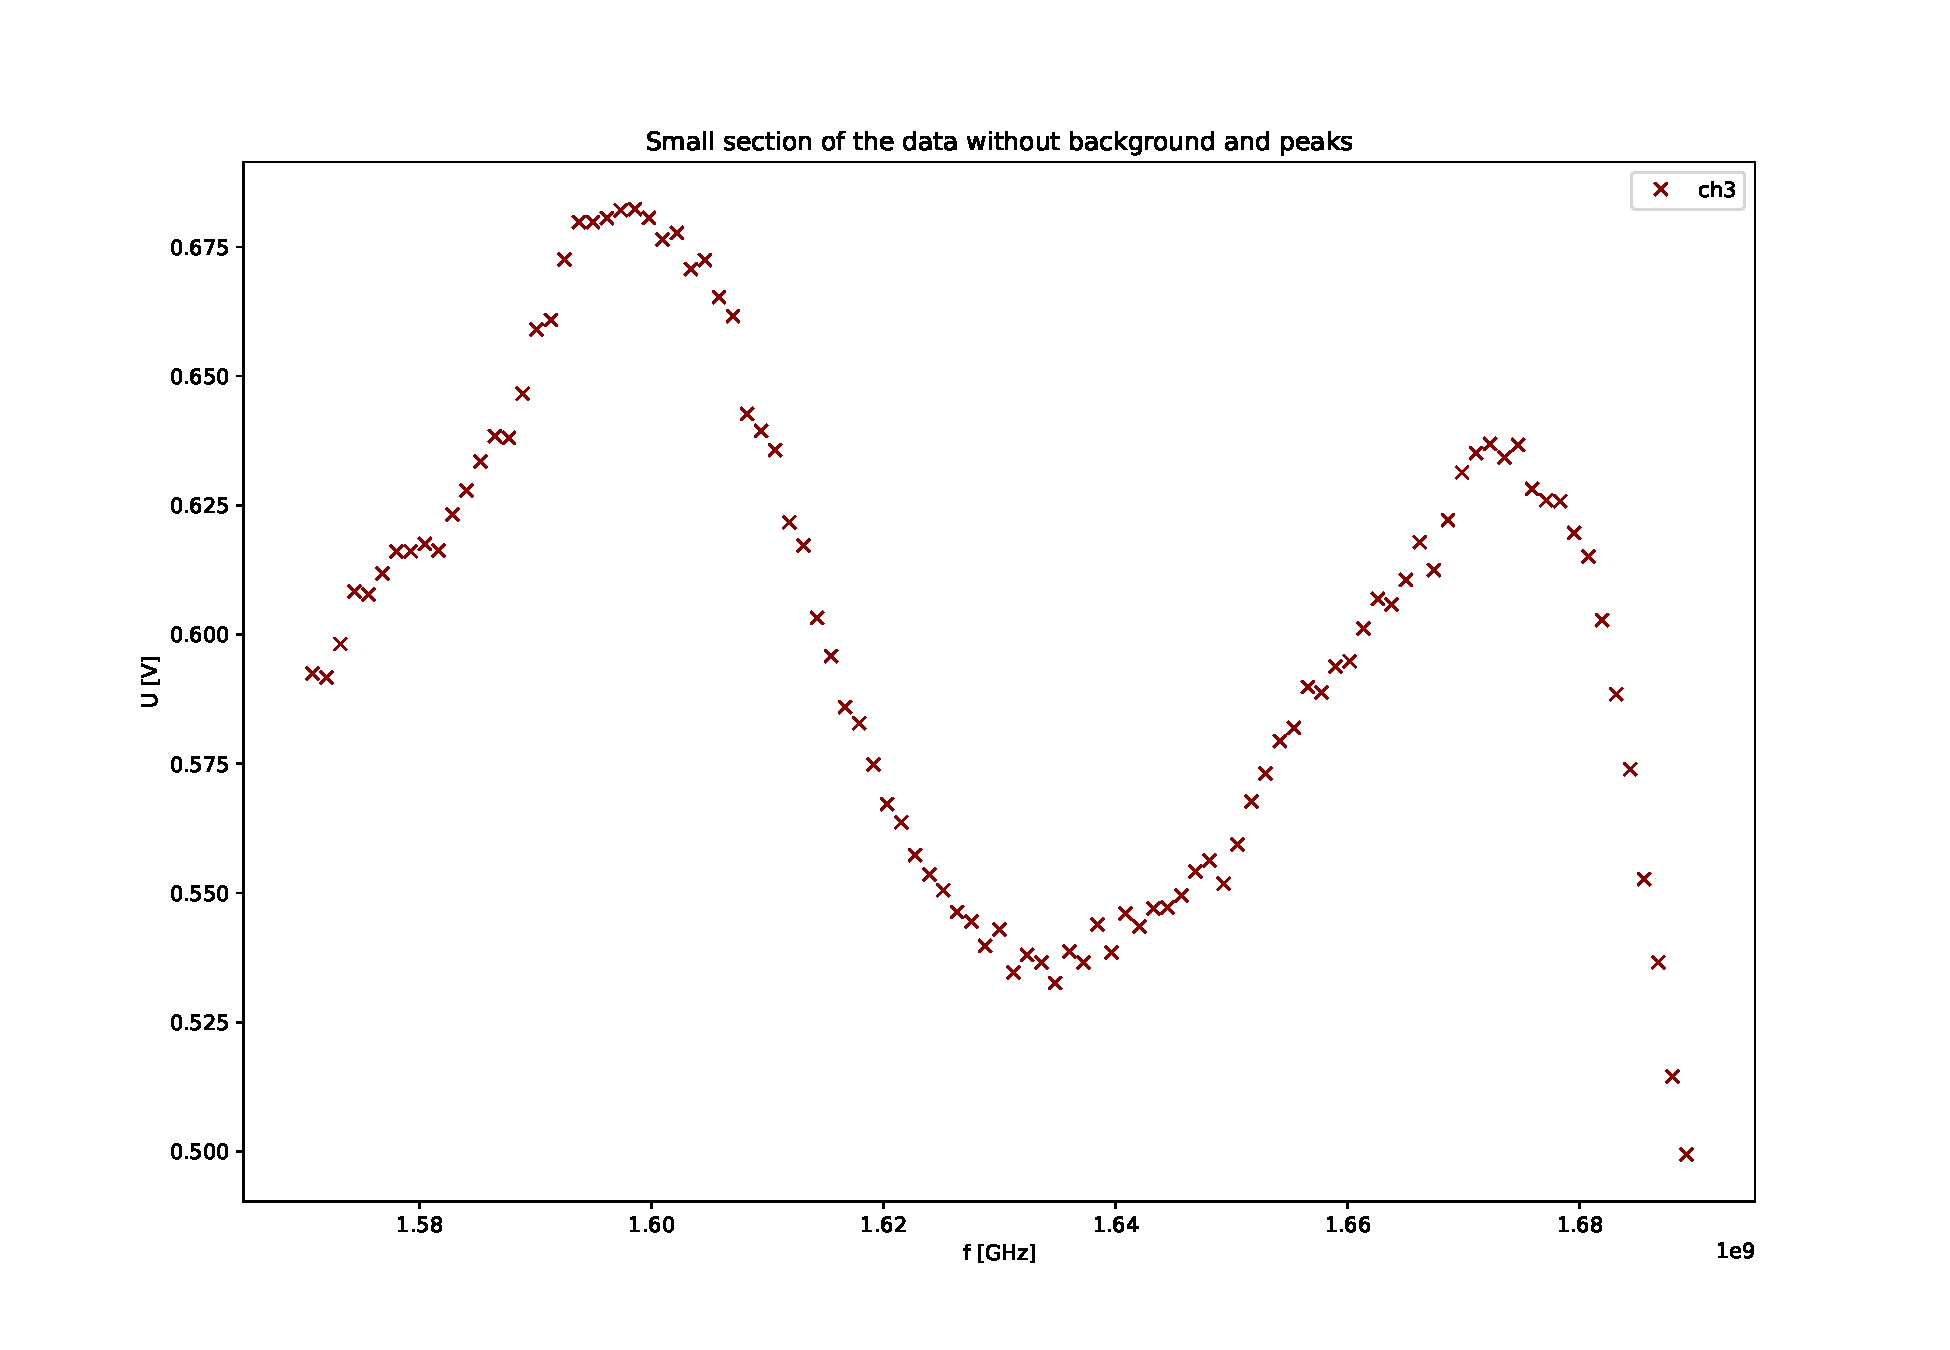
\includegraphics[width=\textwidth]{fig/absorption_cut_1.pdf}
	\caption{The second cut from the fourth dataset, here two peaks are clearly visible}
	\label{fig:absorption_cut_1}
\end{figure}
\begin{figure}[tb]
	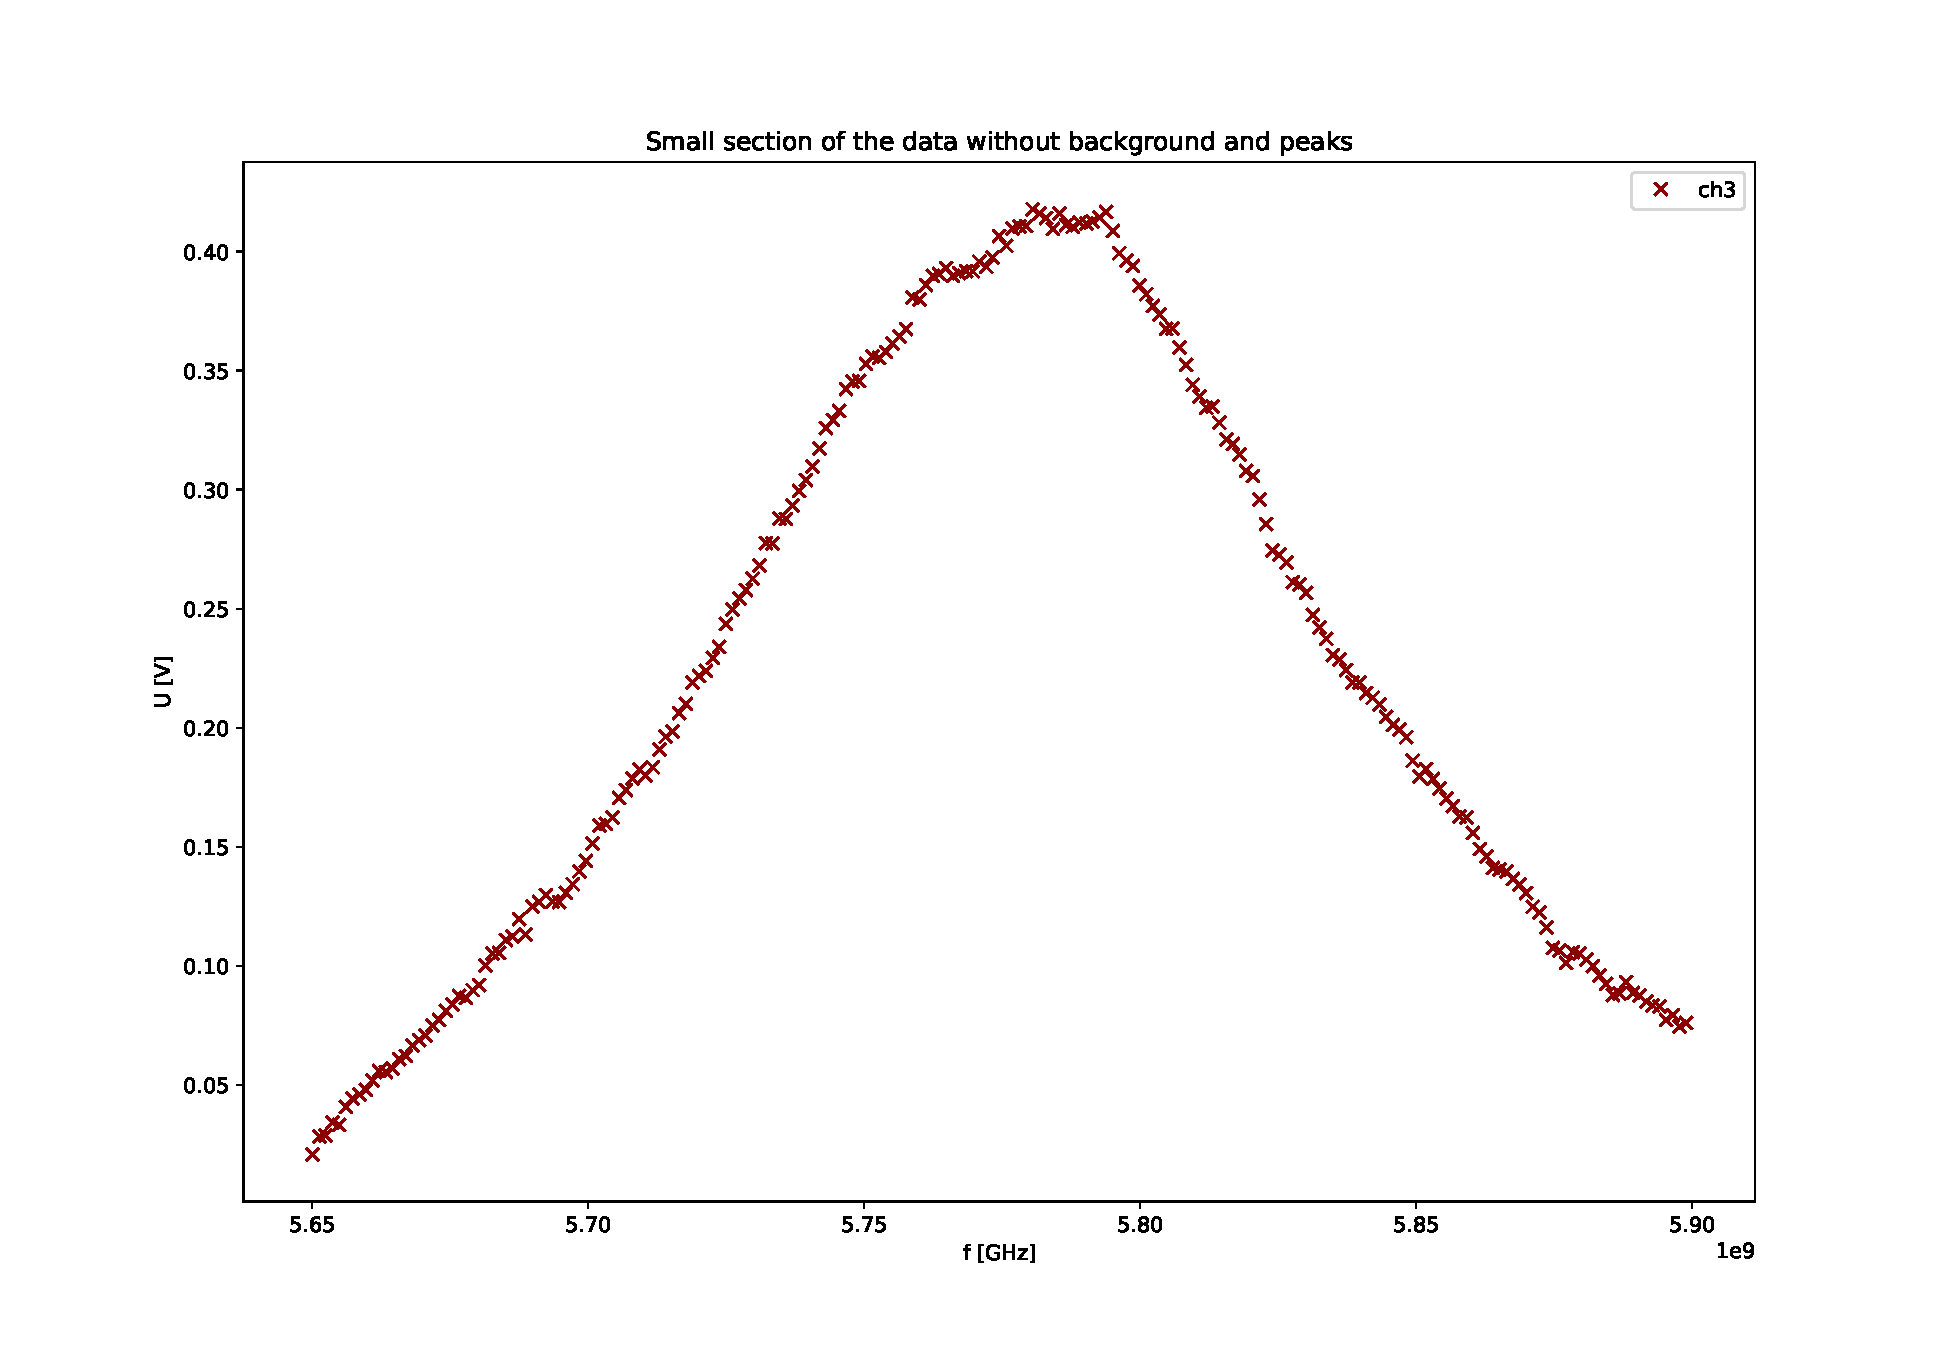
\includegraphics[width=\textwidth]{fig/absorption_cut_2.pdf}
	\caption{The third cut of the fourth dataset. Here one peak is visible}
	\label{fig:absorption_cut_2}
\end{figure}

The Interesting sections are cut from the fourth dataset and can be seen in the figures \ref{fig:absorption_cut_0} to \ref{fig:absorption_cut_2}.

As it was not possible to fit the data in the cases \ref{fig:absorption_cut_0} to \ref{fig:absorption_cut_2} the parameters are estimated by hand.
They are listed in \ref{tab:absorption_peaks}

\begin{table}
	\begin{center}
		\begin{tabular}{|m{10em} m{10em} m{10em}|}
			\hline
			\textbf{Peak} & $f_0$ [GHz] & \textbf{FWHM} [GHz] \\
			\hline\hline
			1 & 2.821 & 0.012 \\
			2 & 2.844 & 0.012 \\
			3 & 1.60 & 0.04 \\
			4 & 1.67 & 0.03 \\
			5 & 5.78 & 0.13 \\
			\hline
		\end{tabular}
		\caption{The location of the resonance absorption peaks}
		\label{tab:absorption_peaks}
	\end{center}
\end{table}

\section{Discussion of Error estimation}
The tasks presented here demand much care in the estimation of errors. The most prominent problem is the subsequent search for and removal of two
consecutive background models. This combines with the need to estimate the conversion factor from scope time to frequency.
The error on the frequency is for this report on the order of 1\%, which compound greatly for all subsequent measurements, because the quantities of
interest are essentially all frequencies. Due to this it is very important to reduce the error in the conversion factor as far as possible. Something
that the data taken for this report did not allow for.

The errors in the Model estimation are difficult to properly propagate into the resulting data points. Again, because the Models are successively
estimated and the data is altered based on the results of the estimation the errors need to be properly handled, which is a non trivial task even for
simple models. The correct propagation of the errors of the estimation of the Gaussian functions for the non-absorption resonance peaks was not done
in this report due to it's complexity. This made any uncertainty estimation beyond that part pointless. On top of this the effect on the choice of
cut-point was not even examined, even though this is an implicit model parameter that needs to be addressed for proper propagation.

As the slope spanned a large set of points, and the data was only affected by the conversion factors uncertainty, The estimation of the parameters is
quite accurate and it's simplicity allows for relatively easy error propagation, which is why that was done.

It is to be noted, that the rising and falling slopes have different characteristics, which is why it is advisable to only select data from either the
rising or the falling slope. The measurements made for this report suggest using the data only from the rising slope as the peaks of channel 2 are
more evenly spaced, while the time distance of the peaks increases toward the end for the falling slope.

The Successive subtraction of correlated models shows how important it is to get many observations that are as uncorrelated as possible and to
separate the data by purpose, as not to cross contaminate the uncertainties with model parameter uncertainties, that are difficult to keep track of.

Over all however, the results agree astoundingly well with the values given in the Documents in preparation for this excercise, despite the amount of
alteration performed on it.
 %\cleardoublepage

    % appendix for more or less interesting calculations
    %\Appendix
    %\chapter*{\appendixname} \addcontentsline{toc}{chapter}{\appendixname}
    % to make the appendix appear in ToC without number. \appendixname = 
    % Appendix or Anhang (depending on chosen language)
    %\section{Erster Abschnitt des Anhangs}
Dies ist der erste ganz tolle Abschnitt des Anhangs. %\cleardoublepage



    % Bibliography
    \TheBibliography

    % BIBTEX
    % use if you want citations to appear even if they are not referenced to: 
    % \nocite{*} or maybe \nocite{Kon64,And59} for specific entries
    %\nocite{*}
    \bibliographystyle{babalpha}
    \bibliography{lit.bib}

    % THEBIBLIOGRAPHY
    %\begin{thebibliography}{000}
    %    \bibitem{ident}Entry into Bibliography.
    %\end{thebibliography}
\end{document}
